% Kai: a typed decision model over evidence
\documentclass[11pt]{article}
\usepackage{../shared/hanzocover}
\usepackage{amsmath, amssymb, amsthm}
\usepackage{booktabs}
\usepackage{graphicx}
\usepackage{xcolor}
\usepackage{enumitem}
\usepackage{array}
\usepackage{listings}
% Custom language definitions for listings
\lstdefinelanguage{Solidity}{
  morekeywords={contract,function,mapping,address,uint256,bytes32,public,private,internal,external,view,pure,returns,event,emit,require,modifier,pragma,solidity,import,struct,enum,if,else,for,while,return,memory,storage,calldata,payable},
  morecomment=[l]{//},
  morecomment=[s]{/*}{*/},
  morestring=[b]",
  sensitive=true,
}
\lstdefinelanguage{GraphQL}{
  morekeywords={query,mutation,subscription,type,input,enum,interface,union,scalar,schema,extend,implements,fragment,on},
  morecomment=[l]{\#},
  morestring=[b]",
  sensitive=true,
}
\lstdefinelanguage{Rust}{
  morekeywords={fn,let,mut,pub,struct,impl,trait,enum,match,if,else,for,while,loop,return,use,mod,crate,self,super,async,await,where,type,const,static,unsafe,extern,ref,move,box,dyn},
  morecomment=[l]{//},
  morecomment=[s]{/*}{*/},
  morestring=[b]",
  sensitive=true,
}
\lstdefinelanguage{Go}{
  morekeywords={func,package,import,type,struct,interface,map,chan,go,defer,select,case,default,if,else,for,range,return,var,const,break,continue,switch,fallthrough},
  morecomment=[l]{//},
  morecomment=[s]{/*}{*/},
  morestring=[b]",
  sensitive=true,
}
\lstdefinelanguage{TypeScript}{
  morekeywords={function,const,let,var,if,else,for,while,return,import,export,from,class,interface,type,enum,async,await,new,this,extends,implements,readonly,private,public,protected,static,abstract},
  morecomment=[l]{//},
  morecomment=[s]{/*}{*/},
  morestring=[b]",
  morestring=[b]',
  sensitive=true,
}
\lstdefinelanguage{JSON}{
  morestring=[b]",
  literate=
    *{0}{{{\color{red}0}}}{1}
    {1}{{{\color{red}1}}}{1}
    {2}{{{\color{red}2}}}{1}
    {3}{{{\color{red}3}}}{1}
    {4}{{{\color{red}4}}}{1}
    {5}{{{\color{red}5}}}{1}
    {6}{{{\color{red}6}}}{1}
    {7}{{{\color{red}7}}}{1}
    {8}{{{\color{red}8}}}{1}
    {9}{{{\color{red}9}}}{1}
    {:}{{{\color{blue}{:}}}}{1}
    {,}{{{\color{blue}{,}}}}{1}
    {\{}{{{\color{blue}{\{}}}}{1}
    {\}}{{{\color{blue}{\}}}}}{1}
    {[}{{{\color{blue}{[}}}}{1}
    {]}{{{\color{blue}{]}}}}{1},
}
\lstdefinelanguage{YAML}{morekeywords={true,false,null},morecomment=[l]{\#},morestring=[b]",sensitive=true}
\lstdefinelanguage{TOML}{morekeywords={true,false},morecomment=[l]{\#},morestring=[b]",sensitive=true}
\lstdefinelanguage{Lean}{morekeywords={theorem,lemma,def,where,by,sorry,exact,simp,omega,rfl,have,let,match,if,then,else,do,return,import,open,namespace,section,end,structure,class,instance,inductive,axiom,variable,noncomputable},morecomment=[l]{--},morestring=[b]",sensitive=true}
\lstdefinelanguage{Move}{morekeywords={module,fun,public,struct,resource,let,if,else,while,loop,return,move,copy,abort,acquires,has,key,store,drop},morecomment=[l]{//},morestring=[b]",sensitive=true}
\lstdefinelanguage{Cairo}{morekeywords={fn,let,mut,struct,enum,impl,trait,if,else,loop,return,use,mod,felt252,u8,u16,u32,u64,u128,u256,bool,ref},morecomment=[l]{//},morestring=[b]",sensitive=true}
\lstdefinelanguage{Circom}{morekeywords={template,signal,input,output,component,var,if,else,for,while,return,include,pragma},morecomment=[l]{//},morestring=[b]",sensitive=true}
\lstdefinelanguage{Noir}{morekeywords={fn,let,mut,pub,struct,impl,trait,if,else,for,while,return,use,mod,constrain,assert},morecomment=[l]{//},morestring=[b]",sensitive=true}
\lstdefinelanguage{Vyper}{morekeywords={def,event,log,self,msg,block,if,else,for,return,assert,raise,pass,import,from,interface,implements},morecomment=[l]{\#},morestring=[b]",sensitive=true}

\usepackage{tikz}
\usetikzlibrary{positioning,arrows.meta,fit,calc}
\usepackage{hyperref}
\hypersetup{colorlinks=true,linkcolor=black,citecolor=blue,urlcolor=blue}
% Identifiers set in typewriter do not hyphenate; let a line stretch instead of
% running into the margin.
\setlength{\emergencystretch}{3em}

% The status of a sentence: a figure from a kept run, a description of code on
% the main branch at the revision on the title page, or a design not yet built.
\newcommand{\meas}{\textcolor{blue!60!black}{\small[measured]}}
\newcommand{\shipped}{\textcolor{purple!70!black}{\small[in the code]}}
\newcommand{\proposed}{\textcolor{orange!70!black}{\small[proposed]}}
% A figure someone else published; we have not reproduced it.
\newcommand{\reported}{\textcolor{gray!70!black}{\small[reported]}}

% Result tables are written by `bench tex` (hanzoai/decision) into tables/:
% harness.tex, languages.tex, capability.tex and speed.tex, each a bare tabular.
% Until a checkpoint is scored, each file is a stub built from \pending.
\newcommand{\pending}[1]{%
  \begin{tabular}{@{}>{\centering\arraybackslash}p{0.8\linewidth}@{}}
  \toprule
  \textcolor{orange!70!black}{\textbf{Pending the final checkpoint.}}\\[2pt]
  \small #1\\
  \bottomrule
  \end{tabular}}

\newcommand{\op}[1]{\texttt{#1}}
\newcommand{\allow}{\textup{\textsc{allow}}}
\newcommand{\ask}{\textup{\textsc{ask}}}
\newcommand{\deny}{\textup{\textsc{deny}}}
\newcommand{\join}{\sqcup}
\newcommand{\pmax}{p_{\max}}

\lstdefinestyle{wire}{basicstyle=\ttfamily\footnotesize,breaklines=true,
  columns=fullflexible,keepspaces=true,frame=single,framerule=0.3pt,
  rulecolor=\color{gray!50},xleftmargin=0.5em,xrightmargin=0.5em}

\theoremstyle{definition}
\newtheorem{definition}{Definition}
\theoremstyle{plain}
\newtheorem{proposition}{Proposition}
\newtheorem{corollary}{Corollary}
\theoremstyle{remark}
\newtheorem{remark}{Remark}

% The cover shows the title alone; the title page adds the subtitle.
\title{Kai: A Typed Decision Model over Evidence}
\author{
    Hanzo AI Research\thanks{Corresponding author: research@hanzo.ai} \\
    \textit{Hanzo Industries Inc (Techstars '17)} \\
    San Francisco, California \\
    \texttt{https://hanzo.ai}
}
\date{2026-09-27 \quad Code at \texttt{hanzoai/decision} \texttt{4bdc2e6}}

\begin{document}

\hanzocoverpage
\title{Kai: A Typed Decision Model over Evidence\\[0.35em]
{\large Factorized choice, typed-variable diffusion, and decisions\\
as versioned programs under deterministic policy}}
\maketitle

\begin{abstract}
\noindent
Agents, controllers and engineering studies ask many small questions of
explicit state. Kai answers them as typed decisions, a \op{choice},
\op{score} or \op{noul} over options the caller lists, returned as a
calibrated distribution with no generated text. Kai is one model on one
checkpoint line: a multilingual encoder, adapters that bring sensor streams
with their metadata, audio, images and video into it, and a typed-variable
decoder. Options are encoded alone and scored against the evidence by two
cross-attention blocks, so option count, order and question count are not
bounded by one sequence; \op{noul} is label-symmetric by construction,
\op{score} a cumulative-link model, and a large choice is narrowed by
retrieval that keeps the mass it cuts. A program's dependent questions are
typed variables, decoded as masked slots, refined in waves bounded by
dependency depth and projected exactly onto the program's rules. Programs are
versioned DAGs whose verdicts join a deterministic policy on
$\allow < \ask < \deny$, so no model loosens policy, and each run is a hashed
package that replays, diffs, refreshes and says what flips the decision. Kai
trains in pure Rust, bf16 over F32 masters, as local SGD across Metal, CUDA and
ROCm machines, on data classed by license and held behind a contamination
barrier. We report what went wrong: our first stage-A run lost the encoder's
ability to relate two texts, and we give the measurements, the cause and the
fix. Results against Laya and TypeSafe's Jev on a frozen 62-suite harness, on
capabilities they lack by construction, and on speed are written into the
paper by the benchmark that measures them.
\end{abstract}

\clearpage
\tableofcontents
\clearpage

\section{Introduction}
\label{sec:intro}

Agents ask the same small questions thousands of times per session: which
context the next turn sees, which tool fits, whether a command may
run~\cite{jevnote}. A generative model answers in prose with no probability to
threshold; a fixed rule sees only what its author foresaw. A \emph{typed
decision} sits between: the caller states a question, lists the admissible
answers and passes the evidence, and the model returns a distribution over
exactly those answers, which can be type-checked, thresholded, logged and
replayed.

Three planes: the \emph{generative} writes (Zen), the \emph{decision} answers
typed questions over evidence (Kai), and the \emph{policy} is deterministic,
written by people, and final. A decision is a program, not a prompt
(Figure~\ref{fig:program}): Zen reasons inside it, Kai judges, code and solvers
compute, policy and people hold authority, and each run leaves a package.

% Decision as text against decision as a program.
\begin{figure}[t]
\centering
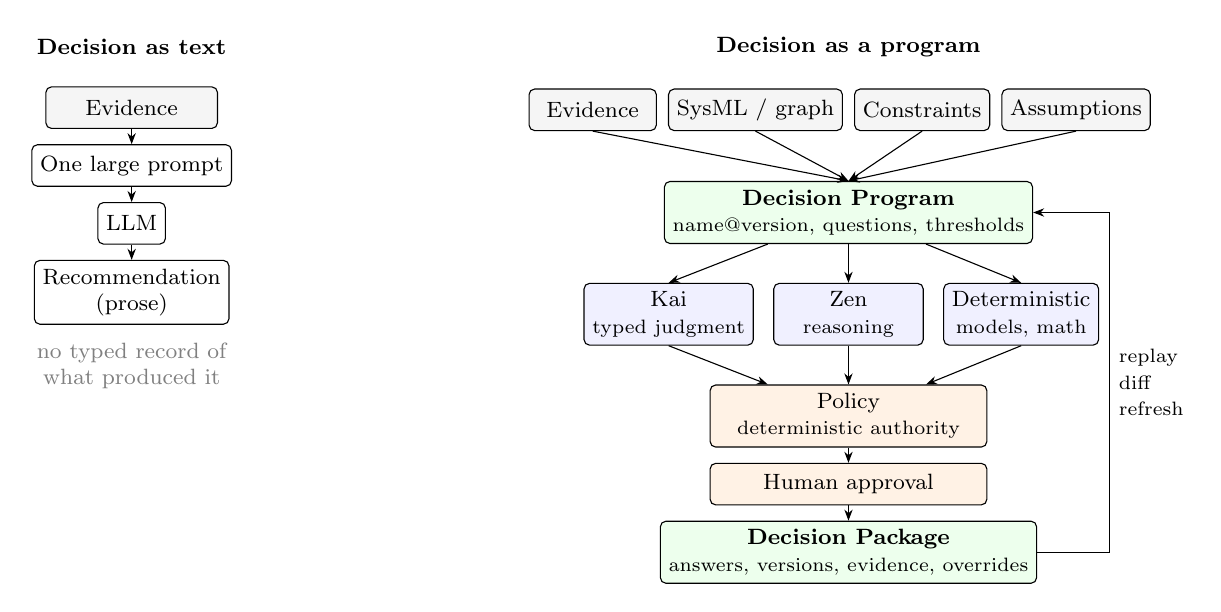
\begin{tikzpicture}[
  font=\footnotesize,
  box/.style={draw, rounded corners=2pt, align=center, minimum height=1.5em,
              inner sep=3pt, fill=white},
  src/.style={box, fill=gray!8, minimum width=6.2em},
  exec/.style={box, fill=blue!6, minimum width=5.4em},
  auth/.style={box, fill=orange!10, minimum width=10em},
  arr/.style={-{Stealth[length=4pt]}, thin},
  node distance=0.55em and 1.2em]

% Left: the decision as text.
\node[font=\footnotesize\bfseries] (lt) {Decision as text};
\node[src, below=0.8em of lt] (le) {Evidence};
\node[box, below=of le] (lp) {One large prompt};
\node[box, below=of lp] (ll) {LLM};
\node[box, below=of ll] (lr) {Recommendation\\(prose)};
\draw[arr] (le) -- (lp);
\draw[arr] (lp) -- (ll);
\draw[arr] (ll) -- (lr);
\node[below=0.3em of lr, text=gray, align=center] {no typed record of\\what produced it};

% Right: the decision as a program.
\node[font=\footnotesize\bfseries, right=17em of lt] (rt) {Decision as a program};
\node[src, minimum width=4.6em, anchor=north east] (e2) at ([xshift=-0.2em,yshift=-0.8em]rt.south) {SysML / graph};
\node[src, minimum width=4.6em, anchor=north west] (e3) at ([xshift=0.2em,yshift=-0.8em]rt.south) {Constraints};
\node[src, minimum width=4.6em, left=0.4em of e2] (e1) {Evidence};
\node[src, minimum width=4.6em, right=0.4em of e3] (e4) {Assumptions};
\coordinate (srow) at (e2.south -| rt);
\node[box, fill=green!7, minimum width=12em, below=1.8em of srow] (dp)
  {\textbf{Decision Program}\\\scriptsize name@version, questions, thresholds};
\foreach \e in {e1,e2,e3,e4} \draw[arr] (\e.south) -- (dp.north);

\node[exec, below=1.4em of dp] (zen) {Zen\\\scriptsize reasoning};
\node[exec, left=0.7em of zen] (kai) {Kai\\\scriptsize typed judgment};
\node[exec, right=0.7em of zen] (det) {Deterministic\\\scriptsize models, math};
\draw[arr] (dp) -- (kai.north);
\draw[arr] (dp) -- (zen.north);
\draw[arr] (dp) -- (det.north);

\node[auth, below=1.4em of zen] (pol) {Policy\\\scriptsize deterministic authority};
\draw[arr] (kai.south) -- (pol);
\draw[arr] (zen.south) -- (pol);
\draw[arr] (det.south) -- (pol);
\node[auth, below=of pol] (hum) {Human approval};
\node[box, fill=green!7, minimum width=12em, below=of hum] (pkg)
  {\textbf{Decision Package}\\\scriptsize answers, versions, evidence, overrides};
\draw[arr] (pol) -- (hum);
\draw[arr] (hum) -- (pkg);
\draw[arr] (pkg.east) -- ++(2.6em,0) |- node[pos=0.25, right, align=left]
  {\scriptsize replay\\\scriptsize diff\\\scriptsize refresh} (dp.east);
\end{tikzpicture}
\caption{Left: the usual shape, in which one generative call turns evidence
into a recommendation and nothing typed records how. Right: Hanzo Decision.
A versioned program states the questions; Kai answers the bounded judgments,
Zen the open reasoning, and deterministic models the arithmetic; policy and a
person hold authority; every run produces a package that can be replayed,
compared with another run, and refreshed.}
\label{fig:program}
\end{figure}


Two decision models exist to compare against, and both are baselines, never
Kai revisions. Laya~\cite{laya} is a family of open encoder checkpoints that
pack the question, every option and the state into one sequence; TypeSafe's
Jev~\cite{typesafejev} is a hosted model behind OpenRouter's Decisions
API~\cite{openrouterdecisions}. Status tags: \meas{} run by us, with the kept
artifact named; \reported{} published by others; \shipped{} on the main branch
of \texttt{hanzoai/decision} at the revision on the title page; \proposed{}
designed, not built.

\paragraph{Contributions.}
\begin{enumerate}[leftmargin=1.5em]
  \item \textbf{One model}: an evidence record for any modality with its
    sensor metadata, adapters into one encoder's width, and evidence, questions
    and options each encoded once per session; one checkpoint line trained in
    stages
    (Section~\ref{sec:model}).
  \item \textbf{Factorized choice}: options encoded alone and scored against
    shared evidence by two cross-attention blocks, a law per type, and
    retrieval that keeps the mass it cuts, so option count, order and question
    count are not bounded by one sequence (Section~\ref{sec:factor}).
  \item \textbf{Typed-variable diffusion}: a program's questions as masked
    slots decoded jointly over the program graph, refined in waves bounded by
    its depth and projected exactly onto its rules (Section~\ref{sec:diffusion}).
  \item \textbf{A training system} in pure Rust: local SGD with an outer
    Nesterov step across Metal, CUDA and ROCm machines, bf16 deltas with error
    feedback, bit-identical resume, token-budgeted batches under a memory
    floor, license classes and a contamination barrier
    (Section~\ref{sec:training}).
  \item \textbf{What went wrong}: stage A's encoder stopped relating two texts;
    the measurements, the ablations that locate the cause, and the fix; and how
    much of the typed-decisions test set Laya's checkpoint had seen in near
    form (Section~\ref{sec:findings}).
  \item \textbf{Policy precedence} as a lattice join, with a proof that
    enforcing a model only adds friction, and \textbf{programs and packages}
    that replay, diff, refresh and say what flips a decision, with SysML~v2
    import and an engineering knowledge graph
    (Sections~\ref{sec:authority} and~\ref{sec:programs}).
  \item \textbf{Benchmarks} of accuracy on a frozen harness, of capabilities
    the baselines lack by construction, and of speed, each table written by
    the command that measures it (Section~\ref{sec:evaluation}).
\end{enumerate}

\paragraph{What is claimed.}
The baselines' structural limits are measured: Laya rejects every question of
1{,}000 or more options and Jev every question over 255; answering five
dependent questions independently, Laya breaks one of the program's rules in
64\% of states and Jev in 25\%; reordering 16 options changes Laya's top
answer on 25.5\% of questions \meas{} (\texttt{hanzoai/benchmarks}
\texttt{4e57fb2}). The final checkpoint's numbers enter only through the
tables of Section~\ref{sec:evaluation}, which print ``pending'' until it is
scored; no sentence states them, and the first stage-A run's numbers appear
only where Section~\ref{sec:findings} explains what went wrong. Kai trains on the
train splits of the harness's sources behind a barrier against its test
states, so a lead on a suite whose baseline never saw its source is
in-distribution for Kai, and Section~\ref{sec:limits} says what that does not
show.

\section{Typed decisions}
\label{sec:decisions}

\begin{definition}[Typed question]
A typed question is a triple $q = (\tau, \iota, C)$ of a type
$\tau \in \{\op{choice}, \op{score}, \op{noul}\}$, an instruction $\iota$ in
natural language, and an ordered list of options
$C = (c_1, \dots, c_k)$, each a label with a description.
A \op{choice} selects one of $k \ge 1$ unordered labels; a \op{score} selects
one of $k$ ordered levels $0, \dots, k-1$; a \op{noul} is a predicate, $k = 2$,
with sides $(\op{false}, \op{true})$ whose descriptions the caller may
override.
\end{definition}

\begin{definition}[Answer]
An answer to $q$ over evidence $E$ is a distribution $p \in \Delta^{k-1}$ over
$C$. A \op{choice} reports $\arg\max_i p_i$, a \op{score} the expected level
$\bar\ell = \sum_i i\, p_i$ with a legend, a \op{noul} $p_{\op{true}}$; every
answer also carries $p$.
\end{definition}

$(q, E)$ and the model revision determine $p$, so a decision replays.

\subsection{What an answer is sure of}
\label{sec:confidence}

Three summaries of $p$ are in use under the name \op{confidence}, and they are
different numbers: the top probability $\pmax = \max_i p_i$; the rescaled
maximum
\begin{equation}
  \kappa = \frac{k\,\pmax - 1}{k - 1}, \qquad k \ge 2,
  \label{eq:kappa}
\end{equation}
which is 0 at the uniform distribution and 1 at a point mass, reported by Jev
and OpenRouter~\cite{laya,openrouterdecisions}; and one minus normalised
entropy, $h = 1 - H(p)/\ln k$, reported by the Laya runtime~\cite{laya}.

\begin{proposition}
\label{prop:kappa}
For fixed $k$, $\kappa \ge t \iff \pmax \ge \bigl(1 + t(k-1)\bigr)/k$.
\end{proposition}
\begin{proof}
Equation~\eqref{eq:kappa} is affine and increasing in $\pmax$ for $k \ge 2$.
\end{proof}

So $\kappa \ge 0.5$ asks for $\pmax \ge 0.75$ on a \op{noul}, $0.67$ on a
three-way and $0.55$ on a ten-way choice: one threshold, a different risk per
arity; $h$ orders answers differently again. For $p = (0.05, 0.15, 0.80)$, $\kappa = 0.70$ and
$h = 0.44$; a gate at 0.5 passes under one and abstains under the other.

\paragraph{The convention we fix.}
Every backend behind \op{/v1/decisions} reports \op{confidence} as $\kappa$,
so a threshold written for Jev means the same when Kai answers, and adds
\op{answer\_confidence} $= \pmax$. A Decision Program writes abstention
thresholds against $\kappa$ and \op{noul} thresholds against $p_{\op{true}}$,
and names the calibration they were set against (Section~\ref{sec:programs})
\shipped.

\section{Kai}
\label{sec:model}

Kai is one model: a multilingual text encoder, adapters that bring any other
evidence into its width, a factorized option head, and a typed-variable decoder
over a program's questions (Figure~\ref{fig:kai}). It maps evidence $E$, a
typed question and, inside a program, other questions' answers to a
distribution over the question's options. Everything in this section is in the
\texttt{kai} crate \shipped; what is trained, and when, is
Section~\ref{sec:training}.

% Kai: encoder, evidence adapters, decoder. Every box is in the code.
\begin{figure}[t]
\centering
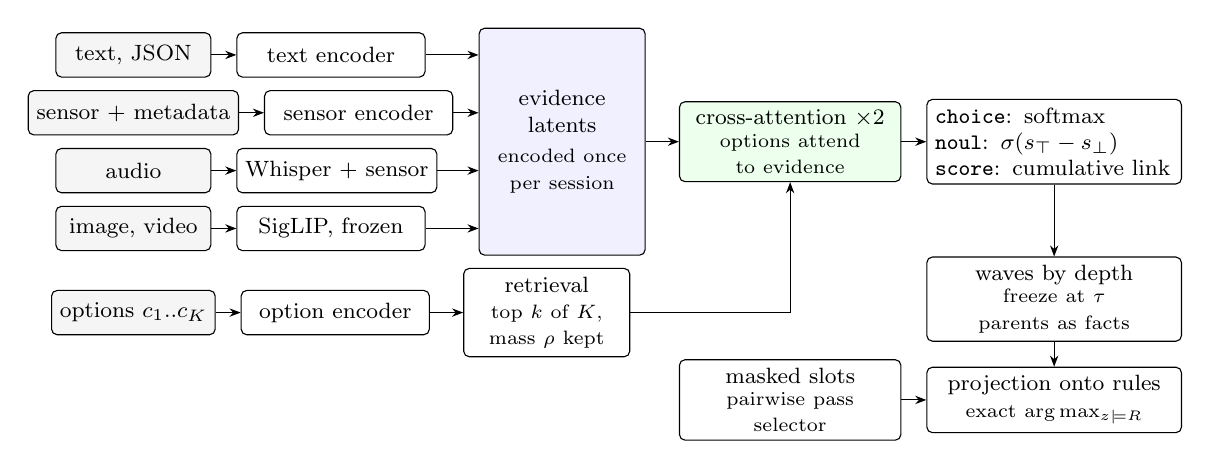
\begin{tikzpicture}[
  font=\footnotesize,
  box/.style={draw, rounded corners=2pt, align=center, inner sep=3pt,
              minimum height=1.6em, fill=white},
  src/.style={fill=gray!8, minimum width=5.6em},
  enc/.style={minimum width=6.8em},
  arr/.style={-{Stealth[length=4pt]}, thin},
  node distance=0.45em and 0.9em]

% evidence and its encoders
\node[box, src] (txt) {text, JSON};
\node[box, src, below=of txt] (sen) {sensor + metadata};
\node[box, src, below=of sen] (aud) {audio};
\node[box, src, below=of aud] (img) {image, video};
\node[box, enc, right=of txt] (etxt) {text encoder};
\node[box, enc, right=of sen] (esen) {sensor encoder};
\node[box, enc, right=of aud] (eaud) {Whisper + sensor};
\node[box, enc, right=of img] (eimg) {SigLIP, frozen};
\foreach \a/\b in {txt/etxt, sen/esen, aud/eaud, img/eimg} \draw[arr] (\a) -- (\b);
\node[box, fill=blue!6, minimum height=8.2em, text width=5.4em,
      right=1.2em of $(esen.east)!0.5!(eaud.east)$] (H)
  {evidence latents\\[3pt]\scriptsize encoded once\\\scriptsize per session};
\foreach \e in {etxt, esen, eaud, eimg} \draw[arr] (\e.east) -- (H.west |- \e);

% options
\node[box, src, below=1.4em of img] (opt) {options $c_1..c_K$};
\node[box, enc, right=of opt] (eopt) {option encoder};
\node[box, right=1.2em of eopt, text width=5.4em] (ret)
  {retrieval\\\scriptsize top $k$ of $K$, mass $\rho$ kept};
\draw[arr] (opt) -- (eopt);
\draw[arr] (eopt) -- (ret);

% head
\node[box, fill=green!7, right=1.2em of H, text width=7.4em] (xa)
  {cross-attention $\times 2$\\\scriptsize options attend\\\scriptsize to evidence};
\draw[arr] (H) -- (xa);
\draw[arr] (ret.east) -| (xa.south);
\node[box, right=0.9em of xa, text width=8.6em, align=left] (law)
  {\op{choice}: softmax\\\op{noul}: $\sigma(s_{\top} - s_{\bot})$\\\op{score}: cumulative link};
\draw[arr] (xa) -- (law);

% refinement
\node[box, below=2.6em of law, text width=8.6em] (wave)
  {waves by depth\\\scriptsize freeze at $\tau$\\\scriptsize parents as facts};
\node[box, below=0.9em of wave, text width=8.6em] (proj)
  {projection onto rules\\\scriptsize exact $\arg\max_{z \models R}$};
\node[box, left=0.9em of proj, text width=7.4em] (sel)
  {masked slots\\\scriptsize pairwise pass\\\scriptsize selector};
\draw[arr] (law) -- (wave);
\draw[arr] (wave) -- (proj);
\draw[arr] (sel) -- (proj);
\end{tikzpicture}
\caption{Kai: a text encoder, evidence adapters and a typed-variable decoder.
Evidence is encoded once per session; options are encoded alone, narrowed by
retrieval above $k$, and scored against the evidence by two cross-attention
blocks under the question type's law; a program's dependent questions are
decoded as masked slots, refined in waves by depth, and projected onto its
rules. Every box is in the code; the adapters train in stage B and the slot
decoder in stage C.}
\label{fig:kai}
\end{figure}


\subsection{Evidence}
\label{sec:evidence}

\begin{definition}[Evidence]
An evidence record is a tuple
\[
  e = (\mathit{id}, \mathit{modality}, t, \mathit{source}, \mathit{frame},
  \mathit{unit}, \mathit{sensor}, \mathit{uncertainty}, \mathit{quality},
  \mathit{provenance}, \mathit{payload})
\]
of an identifier the state's text may cite, a modality (eighteen named, any
other a $\op{Custom}(\cdot)$), a time span, the payload's frame and unit, sensor
metadata (sensor, location, calibration date and validity, limits, and per
channel a name, unit, calibration, error bound and quality), an uncertainty (a
standard deviation, an interval or a quality grade), a quality flag (valid,
degraded or expired, with a loss share), the producer with its inputs, and a
payload: text, JSON, numeric channels with a rate or timestamps, bytes, frames,
a grid, a vector, points, or a URL the caller resolves. A decision's evidence is
the state plus a set of records.
\end{definition}

A new sensor needs an adapter, not a new model, and a number is never serialized
as prose: 43.2\,\textdegree C, 43.2\,psi and 43.2\,mm/s differ by their unit,
and an expired calibration weakens the record. The adapter follows from the
payload's form. Text and JSON go through the text encoder, pooled. Numeric
channels go through a sensor encoder: patches of the series as points, log
bands and statistics, six summary tokens per channel (instant, windows, trend,
events, baseline, forecast), and each channel's metadata line through the text
encoder. Audio takes two paths, Whisper-base~\cite{radford2023whisper}, frozen,
for what is said and the sensor encoder over the waveform for how it sounds;
images and thermal or radar grids go through SigLIP~\cite{zhai2023siglip},
frozen; video becomes appearance, motion and event tokens from SigLIP per
frame, never unbounded frame tokens; vectors and point clouds go through a
projector. Every token gains embeddings for its modality, quality, descriptor
(time, uncertainty) and metadata line. The context the option head attends to
is the text encoder's tokens followed by the evidence tokens; retrieval's query
stays the text's. Forecasts from time-series
models~\cite{das2024timesfm,ansari2024chronos} enter as records, not answers.

A checkpoint that declares no evidence answers bit for bit as a text-only one,
so adapters can be added to a trained line.

\paragraph{Encode once.}
A question's context takes one of two layouts, a checkpoint field. In the
first, each question is one sequence with the state inside it,
\[
  \texttt{[CLS]}\ \langle\tau\rangle\ \texttt{question:}\ \iota\
  \texttt{[SEP]}\ s\ \texttt{[SEP]},
\]
cut at the context length by dropping the state's tail. In the \emph{shared}
layout the state is encoded once, \texttt{[CLS]}~$s$~\texttt{[SEP]}, for every
question put to it, each question is its own sequence, and an option's tokens
attend to the question's tokens with its evidence and to the state's tokens
under one softmax, the state's keys and values projected once and gathered per
row. The weights are the same, so a stage may switch layouts from any
checkpoint: the stage-A runs use the first, stage C the shared one. Either way
options never share the context's token budget, and an option's tokens depend
on its text alone, so every distinct option in a batch is encoded once for all
the questions that list it; inside a program session every evidence record,
question and option is encoded once whatever the number of refinement passes.
Keeping latents across calls, keyed by content hash per changed evidence state
and per program version, is \proposed.

\subsection{Factorized choice}
\label{sec:factor}

Let $C$ be the tokens a question's options attend to, each with the question
type's learned embedding $e_\tau$ added, and $O_i \in \mathbb{R}^{L_i\times d}$
the token states of option $i$, encoded alone as
\texttt{[CLS]}~$c_i$~\texttt{[SEP]}. Two pre-norm cross-attention blocks, in
which option tokens attend to the context and to nothing else, give
$X_i = B_2(B_1(O_i + e_\tau, C), C)$; with $v_i$ the mean of $X_i$,
\begin{equation}
  s_i = w^{\top}\,\mathrm{GELU}\bigl(W\,\mathrm{LN}(v_i) + b\bigr).
\end{equation}
The type fixes the law, at a temperature $T$ fitted per type and option-count
bucket on held-out data:
\begin{itemize}[leftmargin=1.5em]
  \item \op{choice}: $p_i = \operatorname{softmax}_i(s_i/T)$.
  \item \op{noul}: $p_{\op{true}} = \sigma\bigl((s_{\op{true}} -
    s_{\op{false}})/T\bigr)$, each side scored with its own description.
  \item \op{score}: a cumulative-link model~\cite{mccullagh1980} over levels
    $0..k-1$ with cutpoints $\theta_1 < \dots < \theta_{k-1}$ and
    $P(y < j) = \sigma(\theta_j - \eta)$. The location $\eta = a^{\top}
    \mathrm{std}(\bar v - c)$ reads the mean of the state-aware level vectors
    less a running center $c$; the cutpoints read the level texts alone, a base
    $b^{\top}\mathrm{std}(\bar o)$ and gaps
    $\theta_{j+1} - \theta_j = \operatorname{softplus}(g^{\top}
    [\mathrm{std}(\bar o_j); \mathrm{std}(\bar o_{j+1})])$, with $\bar o_j$ the
    mean of $O_j$ and $\mathrm{std}$ each vector at zero mean and unit variance.
    The likelihood is computed in log space,
    $\log P(y = j) = \log\sigma(\theta_{j+1} - \eta) + \log\sigma(\eta -
    \theta_j) + \log\sigma(g_j)$, which is exact and never a difference that
    rounds to zero.
\end{itemize}
The scorer and the ordinal layers compute in F32 whatever the encoder's dtype:
what decides is a difference of two outputs that can share an offset far larger
than it (Section~\ref{sec:other}).

\begin{proposition}[Symmetry]
\label{prop:symmetry}
For any weights, permuting a question's options permutes $p$ the same way, and
exchanging the texts of a \op{noul}'s sides maps $p_{\op{true}}$ to
$1 - p_{\op{true}}$.
\end{proposition}
\begin{proof}
$s_i$ depends on $c_i$ and $C$ alone, and softmax is permutation equivariant;
the exchange swaps $s_{\op{true}}$ and $s_{\op{false}}$, and
$\sigma(-x) = 1 - \sigma(x)$.
\end{proof}

Laya has neither: its options share one sequence, in order, and each is read at
a marker token whose context includes the options before it.

\paragraph{Retrieval.}
A choice with more than $k$ options, a checkpoint field (32 in the first stage-A
run, 160 since), is narrowed first. The sum of the context's first tokens and
each option's mean token are projected, each less a running center, to unit
vectors $u$ and $r_i$, and
$\pi = \operatorname{softmax}_i(e^{\gamma}\langle u, r_i\rangle)$ with $\gamma$
learned. The head scores the top $k$ under $\pi$, a set $S$, and the rest keep
their retrieval probability:
\begin{equation}
  p_i = \begin{cases} (1-\rho)\,\operatorname{softmax}_{j \in S}(s_j/T)_i & i \in S,\\
  \pi_i & i \notin S,\end{cases}
  \qquad \rho = \sum_{i \notin S} \pi_i ,
\end{equation}
so the mass beyond the top $k$ is kept, not renormalised away, and the head
costs $O(k)$ per question for any option count. A running center moves 1\% of
the way to each training batch's mean input after its step and takes no
gradient; without it, encoder states' shared offset gave every context nearly
the same query (Section~\ref{sec:other}).

\subsection{Typed-variable diffusion}
\label{sec:diffusion}

A program's questions depend on each other, and answered independently they
can break its rules: approving an invoice flagged as a duplicate.

\begin{definition}[Typed variables]
A program's questions are variables $Z = (Z_v)_{v \in V}$, each with a finite
domain $D_v$ (labels, levels, or a \op{noul}'s sides), with a dependency DAG
$G$ on $V$ and rules $R$, each on two answers:
$Z_a = i \Rightarrow Z_b = j$, or $\lnot(Z_a = i \land Z_b = j)$.
\end{definition}

The decoder predicts masked slots jointly: for a masked set $M \subseteq V$,
\begin{equation}
  p_\theta(Z_M \mid E, Z_{V\setminus M}, G) = \prod_{v \in M}
  p_\theta(Z_v \mid E, Z_{V\setminus M}, G).
\end{equation}
A slot is its question's mean token plus a value: a learned mask vector while
its answer is unknown, else the known option's mean token through a linear map.
Decoder layers let each slot attend to the others, with a learned per-head bias
for a parent, a child, any other slot, and itself when its answer is shown,
beside a null key of value zero, and then to the evidence latents. The last
read is the variable's message; through a map that starts at zero it is added
to the query tokens of the variable's options, which the factorized head then
scores against the question and the evidence. A variable with nothing else to
read gets a message of exactly zero, so one variable alone is the factorized
head, and a new decoder answers as the checkpoint it starts from (tested to
$10^{-5}$). For a shown slot the distribution revises the answer shown, and
$1 - p(\text{shown})$ flags it.

Training (stage C) hides variables by one of three patterns: $\lceil r n\rceil$
of $n$ at random with $r \sim U(0, 1]$, absorbing-state discrete
diffusion~\cite{austin2021d3pm} over typed variables rather than tokens; a node
and all its descendants; or only the descendants. It tests 15\% of the shown
answers, half of those shown wrong, so the model learns to revise a wrong
answer and keep a right one. The loss is log loss plus Brier score over hidden
and tested variables, plus the mean probability that the joint state breaks a
rule: $q(a)(1 - q(b))$ for $a \Rightarrow b$, $q(a)\,q(b)$ for
$\lnot(a \land b)$. Every program of two or more variables gains a \op{defer}
variable reading all the others, whose gold is to act when every answer is
clear (top probability at least 0.9) and to defer otherwise.

\paragraph{Refinement.}
One scheduler serves any model that answers a set of questions given known
answers: the decoder with known answers as visible slots, or the factorized
head with a node's known parents added to its state as typed facts. Passes are
spent on uncertainty.
\begin{enumerate}[leftmargin=1.5em]
  \item Pass 1 predicts every variable with nothing known and freezes those
    whose top probability reaches $\tau$.
  \item Waves by dependency depth: a variable settles once frozen, a root, or
    re-asked; each wave asks, once, every unsettled variable whose parents have
    all settled, and freezes again.
  \item Each unfrozen variable keeps its top $m$ candidates. One more pass asks
    each unfrozen variable's unfrozen children with the variable set to each
    candidate, giving pairwise terms
    $\log p(\text{child} \mid \text{node} = c) - \log p(\text{child})$;
    variables sharing a child are set in different jobs, so each term
    conditions on one variable alone.
  \item A selector takes the joint answer over the candidates of highest
    log-probability plus pairwise terms that keeps every rule.
  \item A projection onto the rules over the full domains,
    $\hat z = \arg\max_{z \models R} \sum_{v} \log p_v(z_v)$, moves nothing
    when the selection already keeps them.
\end{enumerate}

\begin{proposition}[Depth bounds cost]
\label{prop:depth}
Steps 1 and 2 end within $\operatorname{depth}(G) + 1$ passes, depth counted in
edges, and ask at most $2|V|$ questions; with step 3, refinement takes at most
$\operatorname{depth}(G) + 2$ passes whatever $|V|$.
\end{proposition}
\begin{proof}
Roots and frozen variables are settled after pass 1. If every variable of depth
below $d$ is settled after pass $d$, each of depth $d$ has all parents settled
and is re-asked by pass $d+1$. Each variable is asked in pass 1 and at most once
more. Step 3 is one pass.
\end{proof}

Selection and projection are exact branch and bound, each node's options tried
best first and bounded by the sum of per-variable maxima. Rules between answers
encode graph colouring, so exact selection is exponential on some graphs: the
search stops with an error after $2^{20}$ steps rather than return an answer it
has not proved.

\subsection{One checkpoint line}
\label{sec:checkpoints}

Kai has one checkpoint line, \texttt{hanzoai/kai}, with a revision per training
stage; language, domain, modality and hardware are not product lines. The
encoder is mmBERT-base~\cite{mmbert}, multilingual with 8{,}192 positions,
trained at 1{,}024 tokens; the code runs any ModernBERT-family
encoder~\cite{modernbert}. Kai initializes from Laya's multilingual
weights~\cite{laya}, released under Apache-2.0: the encoder and type embedding
as they are, Laya's two self-attention head layers split into the two
cross-attention blocks, and its marker scorer as the option scorer; retrieval
and the ordinal head start fresh.

\paragraph{Laya, the baseline.}
Laya 0.3.20's three checkpoints are not Kai revisions: English on
ModernBERT-large at a 512-token context, multilingual on mmBERT-base at 1,024,
and a typed-decisions checkpoint, the English one fine-tuned on the
typed-decisions~\cite{typeddecisions} train split. Their joint head packs the
question and each option after a marker token into one sequence with the state,
and a script detector routes non-English states to the multilingual checkpoint.
Hanzo serves their byte-identical weights natively through a Rust port of the
joint head: against Laya's Python reference on 21 recorded states in twelve
languages and all three checkpoints, the largest logit difference is
$2.86\times 10^{-5}$ against an enforced bound of $10^{-4}$, the largest
probability difference $6.2\times 10^{-6}$, and 108 of 108 labels agree
(\texttt{decision/tests/parity.rs}) \meas. Every decision records the weights'
SHA-256 it was answered with.

\paragraph{Runtime.}
Rust on Hanzo's tensor library, \texttt{hanzo-ml}, on CPU in F32 and on Metal,
CUDA and ROCm in bf16. The \texttt{decision} crate serves
\op{POST /v1/decisions} with Kai and Laya in process and Jev through
OpenRouter, one worker per checkpoint draining its queue into shared forward
passes; the \texttt{control} crate runs a program over many states in process
behind a C ABI (Section~\ref{sec:enso}). No Python is on the serving path.

\section{Training}
\label{sec:training}

Kai trains in stages on one checkpoint line, in Rust, on the machines Hanzo
has: an Apple M4 Max (Metal), a DGX Spark (CUDA) and an AMD Strix Halo with a
Radeon 8060S (ROCm), joined over a LAN. Everything in this section is in the
\texttt{train} crate \shipped{} unless marked.

\subsection{Stages}
\label{sec:stages}

\begin{description}[leftmargin=1.5em,style=nextline]
  \item[A, text decisions.] The train splits of the harness's sources; MASSIVE
    in all 51 locales and MASSIVE utterances half in English; CLINC150, XNLI in
    15 languages, SST-5, BoolQ and MNLI; function selection (ToolACE, Glaive,
    Nemotron's tool calling); agent runs judged by hidden tests (resolve, next
    action); Hanzo's own agent sessions and repositories, labelled by outcomes
    (the next tool result, a re-run, a revert, the file a commit changed), never
    by what the agent chose; 1{,}181 skills; jailbreak prompts collected in the
    wild; and robustness transforms of 13 sources (options shuffled, relabelled,
    swapped, subset, near-miss).
  \item[B, evidence.] Every parameter frozen but the adapters, over bearing
    faults, turbofan degradation (C-MAPSS), speech, hydraulic rigs, Monash
    forecasting, network telemetry, UCR series, and generated conflicts
    (camera against telemetry, specification against SysML, an expired
    calibration) whose gold is \op{evidence\_conflict}, not
    \op{decision\_ready}, and \op{human\_review}.
  \item[C, programs.] The typed-variable decoder over whole programs: rules
    mined from typed-decision gold, turbofan and test-rig programs, SysML~v2
    architectures lowered to programs and mutated once per case with the
    decision's change recorded, readiness, trade and test-plan programs,
    closed-form vehicle dynamics, and pairs of real telemetry with generated
    logs; generators hold out templates whole, so validation and test ask new
    programs.
\end{description}

A stage is one JSON file: its initial checkpoint (a hub revision, or a finished
run whose provenance names that stage with every planned batch merged), data
build, admitted license classes, per-suite takes, frozen prefixes, token
budget, retrieval loss weights, $k$, schedule and outer optimizer. Stage A has
run; Section~\ref{sec:findings} is what it taught, and the final stage-A run
follows from it. The B and C data are built and their stage files written;
their trained checkpoints are \proposed.

\subsection{Local SGD across devices}
\label{sec:cluster}

One path trains a stage on one machine or many: local SGD with an outer
Nesterov step, DiLoCo~\cite{douillard2023diloco}. A coordinator owns the plan,
$\theta$ in F32, the outer optimizer, validation and checkpoints, and runs
inside a worker process; other machines join it at any time. Workers pull
batches one at a time, so a faster device takes more, and run AdamW from
$\theta$ for a round's wall time (300\,s). Each then sends
$\Delta_w = \theta_w - \theta$ in bf16 with the tokens it processed, adding
back what bf16 rounding dropped from its previous delta, error
feedback~\cite{seide2014onebit,karimireddy2019ef}. With $\Delta$ the
token-weighted mean of the round's deltas and $g = -\Delta$,
\begin{equation}
  m \leftarrow \mu m + g, \qquad \theta \leftarrow \theta - \eta\,(g + \mu m).
  \label{eq:outer}
\end{equation}
The change to $\theta$ goes out in bf16, $\theta$ moves by exactly what went out
and the remainder joins the next change, so every worker's copy of $\theta$ is
bit-identical to the coordinator's. Deltas are summed in the order workers
joined, never the order their reports arrive, so a run does not depend on
network timing. A batch counts once its delta is merged; a worker that drops
has its unmerged batches requeued. The handshake checks the build (a hash of
the model and training sources and the lock file), the tokenized corpus and the
parameter names.

\begin{proposition}[Outer step]
\label{prop:outer}
If every round's mean delta is the same $\Delta$, the outer step of
Equation~\eqref{eq:outer} tends to $\frac{\eta}{1-\mu}\Delta$.
\end{proposition}
\begin{proof}
$m$ tends to $g/(1-\mu)$, so $\eta(g + \mu m) \to \eta g (1 + \frac{\mu}{1-\mu})
= \frac{\eta}{1-\mu} g$.
\end{proof}

So $(\eta, \mu) = (0.7, 0.9)$ moves $\theta$ by $7\times$ a round's mean delta
wherever rounds agree, and $(1.0, 0.3)$ by $1.43\times$. Section~\ref{sec:collapse}
is why this number matters.

\paragraph{Exactness.}
A checkpoint (every so many batches, each epoch, and the end) is taken at a
round boundary and holds the weights, the outer momentum, its rounding carry,
the merged batches and the round, and each worker's AdamW moments, step and
carry, which a worker of that name gets back when it rejoins. Resuming continues
bit-identically to the uninterrupted run, and with one step a round, $\eta = 1$
and $\mu = 0$, the cluster equals the same rounds replayed in one process bit
for bit, for one and three workers (tested on CPU). int8 deltas halve the bytes
but broke that equivalence by up to $1.3\times10^{-5}$, so deltas stay bf16.

\paragraph{Heterogeneity.}
The first stage-A run merged 91{,}899 batches from the Metal, CUDA and ROCm
machines in one run; in its round 45 they took 757, 465 and 226 steps at
7{,}054, 4{,}226 and 2{,}325 tokens/s \meas. Pilots of one stage on Metal and on
CUDA agree: mean validation accuracy 0.504 and 0.500 over 48 suites, log loss
1.493 and 1.501 \meas. ROCm needed three kernels \texttt{hanzo-ml} lacked there
(comparison, \op{index\_add}, sigmoid); a stage-A delta with the token
embeddings frozen is 250\,MB in bf16, about 2.2\,s each way over the LAN.

\paragraph{Budget and memory.}
Compute is bf16 over F32 masters~\cite{micikevicius2018mixed}. A batch is bounded
by a budget on context tokens, option tokens, option-head query and key tokens,
rows and evidence tokens, and holds one suite, or a mixed share across suites.
A device that cannot hold the budget runs a batch as micro-batches within a
fraction of it with gradients summed (equal to one pass within
$1.5\times10^{-8}$), and a worker exits cleanly under a free-memory floor, read
from \texttt{sysctl} on macOS and \texttt{/proc/meminfo} on Linux, rather than
push a shared machine into swap. Freezing the token embeddings (61\% of the
weights) raised a stage-A pilot from 5{,}181 to 5{,}747 tokens/s and cut peak
memory from 53.7 to 47.3\,GB; grouping options by length cut option padding from
49\% to 14\%; Muon on the 2-D weights ran at 3{,}125 tokens/s with a worse
validation log loss (2.114 against 2.056) and was removed \meas.

\paragraph{Wide choices.}
A choice whose options exceed the budget trains as inference answers it: on a
sample of $k$ options, the gold first, about half the negatives from
retrieval's current top 64 at $\theta$, a quarter the gold's nearest by token
Jaccard, the rest uniform. A draw is a function of the row, epoch, round and
seed, so every worker draws alike. Before this, 42{,}066 of the first stage-A
plan's 213{,}398 batches were one row whose options alone exceeded the budget,
and at about 2.9\,MB per option token of a CPU F32 step one such row took a
machine past its floor at any micro-batch size \meas.

\subsection{Data, licenses and the barrier}
\label{sec:barrier}

A stage's data is a content-addressed build: the same inputs give the same
hash, shards are homogeneous in source, dataset, revision, license class and
transformation, and each record carries its provenance (source, dataset,
revision, class, transformation, task family, language, domain, decision type,
candidate count, scope). The manifest, with each shard's SHA-256, is what the
trainer admits.

\paragraph{License classes.}
GREEN is permissive or ours; YELLOW is third-party model output from closed or
unnamed generators; RED is non-commercial, unstated or restrictive terms. A
record starts at its dataset's class, judged at the upstream source, and only
rises: one of our own transcripts rises to YELLOW with any message recorded from
a closed model. A turn carrying such a message is shown to Kai only as the
person's messages and tool outputs. Classes are recorded facts; which classes
train is the owner's recorded decision, written into every build (on
2026-09-25, all three), so a GREEN-only build is one flag. Evaluation is a role,
not a class: benchmark datasets, every built set's test split, and whatever the
barrier catches never train, and a run asked to admit them refuses.

\paragraph{The barrier.}
Every protected evaluation item is read at a pin: the frozen harness's 9{,}499
states, the extension suites' 82{,}860 test states, the Army demo models, and
the Enso study's workloads (GPQA Diamond, HLE, LiveCodeBench v6, CharXiv,
SWE-bench Pro and Verified, Terminal-Bench 2.0), 98{,}065 items; WordNet, which
the capability suites draw on, is banned outright. A record is caught when
\begin{itemize}[leftmargin=1.5em]
  \item it shares an exact content unit with an item: the state's string leaves
    in order with whitespace squashed and keys ignored, or the first 200 letters
    and digits of any leaf of 200 or more characters;
  \item it carries an item's key, a SWE-bench instance id;
  \item it is a near duplicate: estimated Jaccard of character 5-gram sets at
    least 0.5, from 256 min-hashes~\cite{broder1997resemblance} in 64 LSH bands
    of 4, so a pair at Jaccard $j$ is a candidate with probability
    $1 - (1 - j^4)^{64}$, 0.984 at 0.5, and each candidate is checked on all
    256;
  \item it contains an item: at least 80\% of the item's sampled 50-character
    spans, a span sampled when its hash is 0 mod 16 so both sides sample the same
    windows; an item of 50 or more characters with fewer than four sampled spans
    is contained when a text holds its whole normal form.
\end{itemize}
The last rule exists because the one before it missed two: a harness test email
quoted inside a longer train email, and a harness jailbreak prompt opening a
longer one, reached five records of the first stage-A build. Planted over every set (twenty
items each, verbatim, with a word dropped and two swapped, and inside 1{,}900
characters of transcript), nothing of 50 or more characters reaches a shard; an
item under 50 characters, a MASSIVE or CLINC utterance, is caught only when
equal or near, since phrases that short recur in unrelated text. The build the
final stage-A run reads (\texttt{a3-d7a9a437cf484811}) read 2{,}762{,}444
records and caught 19{,}803: against the harness 14{,}875 near duplicates and 71
containments, against the extension suites 4{,}818 near, 34 exact and 3
contained, and 2 SWE-bench keys; 547 of typed decisions' 1{,}185 train states
were caught near (Section~\ref{sec:overlap}). Its records are 1{,}799{,}005
GREEN, 217{,}727 YELLOW and 713{,}841 RED \meas.

\section{What stage A taught}
\label{sec:findings}

Every figure in this section is \meas{}, from runs whose logs, stage files and
scripts are kept beside the paper in \texttt{data/diagnosis/} or recorded in
\texttt{hanzoai/decision}'s \texttt{LLM.md}.

\subsection{The encoder stopped relating two texts}
\label{sec:collapse}

The first stage-A run started from Laya's multilingual weights and trained one
epoch of the full mixture, 91{,}899 batches over three machines, with the outer
step $(\eta, \mu) = (0.7, 0.9)$, $7\times$ a round's mean delta
(Proposition~\ref{prop:outer}). Validation split in two. Tasks that relate two
texts fell: RAG relevance was 0.625 and BoolQ 0.826 at 2{,}325 batches, 0.482
and 0.668 at 13{,}101, and RAG's log loss sat at $\ln 2$ at every validation
after; from 13{,}101 batches to the end MNLI fell from 0.713 to 0.593 and XNLI
from 0.698 to 0.630. Single-text tasks rose over the same span: AG News from
0.375 to 0.845, emotion from 0.525 to 0.679, MASSIVE from 0.440 to 0.730. On the
frozen harness the checkpoint answered RAG relevance at chance (F32 accuracy
0.480, AUC 0.486, 374 of 400 questions answered relevant), and a ridge probe on
the head's option vectors read relevance at AUC 0.35 where the same probe read
jailbreak at 0.93. Its encoder layers ended 30 to 44\% (relative Frobenius
norm) from their initial weights; the English baseline of the same head,
trained in one process at the same learning rates for 53{,}322 steps, ended 5\%
from its own and kept RAG relevance at 0.682.

\paragraph{Not the data.}
All 155{,}761 RAG training records agree with MS~MARCO's \op{is\_selected}
label, except 281 pairs MS~MARCO itself labels both ways; the classes are
balanced (77{,}955 and 77{,}806), and 76{,}109 queries carry exactly one
selected and one unselected passage. The relabelling transform leaves every
target as it was and the side swap reverses target and option texts together
on all 3{,}995 rows. The barrier removed 339 of 159{,}258 records. Truncation
(contexts of 52 to 250 tokens under a 1{,}024-token limit), the fitted
temperature, the class prior and bf16 were each ruled out.

\paragraph{The encoder, not the head.}
Single-process fits on the RAG shards alone, on Metal, locate the fault:
\begin{itemize}[leftmargin=1.5em]
  \item from Laya's multilingual weights, validation accuracy reached 0.645
    after 229 batches;
  \item from the stage-A checkpoint it stayed at 0.497 and 0.495, training log
    loss at 0.693, chance; 0.522 in F32;
  \item stage A's encoder under the head of the Laya run at 229 batches: 0.517,
    then 0.497, training loss at 0.693;
  \item that run's encoder under stage A's head: 0.662 after 104 batches, the
    training loss falling to 0.45.
\end{itemize}
Measured on the encoders alone, over 200 RAG validation contexts laid out as Kai
lays them and run in F32 by an independent ModernBERT implementation, the mean
cosine similarity between different contexts' mean token states is 0.981 for
stage A against 0.853 for Laya (1 would make every context the same), and
swapping only the query moves the passage tokens' states by 0.085 of their norm
in stage A against 0.34 in Laya and 0.73 in the RAG-trained encoder. Stage A's
encoder had stopped letting one text change how it reads the other.

\paragraph{The cause.}
The outer step alone does not do it: on the RAG shards alone, from Laya's
weights, with $(0.7, 0.9)$, validation read 0.590, 0.532, 0.623 and 0.580,
noisier than plain training and never at chance. One process over the English
mixture does not do it either (the baseline above). The full mixture under the
$7\times$ outer step does. Which part of the mixture drives it would take a
replay of stage A, which we did not run. Two continuations agree. Stage a2
continued stage A with the same outer step and regressed on Metal and CUDA
alike, then diverged in cooldown (training log loss 2.85 to 13.45 while the
learning rate fell to a tenth); stage a3 continued it with $(1.0, 0.3)$ and
inherited the collapse, validation RAG 0.497, BoolQ 0.638, MNLI 0.583 and XNLI
0.600 at 16{,}598 batches while its single-text suites were at their best (AG
News 0.890, emotion 0.831, MASSIVE 0.787), and was stopped.

\paragraph{The fix.}
The final stage-A run starts again from Laya's multilingual weights, over a3's
data (two epochs of the harness's train suites at the English baseline's takes,
the rest of the mixture as replay), with the outer step $(1.0, 0.3)$,
$1.43\times$ a round's mean delta, and validates every 8{,}000 batches so a
repeat shows early. Logging the context similarity above at each validation, a
cheap early warning, is \proposed. The harness decides whether the fix held;
its tables are Section~\ref{sec:accuracy}'s.

\subsection{Laya had seen half the typed-decisions test set, reworded}
\label{sec:overlap}

The barrier caught 547 of the 1{,}185 typed-decisions train states it read, all
as near duplicates (measure 0.50 to 0.97, median 0.61), none exact. Laya's
typed-decisions checkpoint was fine-tuned on the whole train split. Measured
over its 1{,}200 rows with the barrier's measure (a state's string leaves;
numbers ignored), 587 rows sit at Jaccard 0.5 or more from some test state, all
in two of the four workflows (agent traces 298 of 300, invoices 289 of 300); on
the test side, 200 of the 400 states, every agent-trace and every invoice
state, have such a sibling. They are template siblings, not copies:
\begin{itemize}[leftmargin=1.5em]
  \item with numbers included no train state equals a test state; the closest
    pair scores 0.90, and 44 score 0.8 or more;
  \item a caught train row agrees with its nearest test state on 0.406 of the
    questions and on all five in 38 of 587, where random train and test states
    of the same workflow agree on 0.416 and on all five 5.3\% of the time;
  \item the test set shares templates with itself as much: 195 of its 400
    states have another test state at 0.5 or more.
\end{itemize}
One pair: the same task (``Update every service to the patched logging
library.''), agent and constraint; in train one constraint violation and one
irreversible action, gold \emph{harmful}, \emph{human review}, risk 3; in test
none of either and two tool errors, gold \emph{partial}, \emph{observe}, risk 1.
So Laya's typed-decisions checkpoint saw same-wording siblings of half the test
set, with different numbers and different gold, and no near-copy of a test
answer. Stage A's builds drop the 547, so it trains on 638 of the states the
builder reads; from stage a5 an official train split is checked only for exact
copies and keys, so all 1{,}185 train. Whether knowing the templates helps is measured, not assumed:
\texttt{harness/siblings.py} in the benchmark repository scores the 235 test
states without a sibling and the 165 with one apart
(Table~\ref{tab:siblings}). Laya's typed checkpoint scores alike on both
halves, so its lead is not memorized from the siblings; Jev, which never saw
them, is 8 points better without them; and Kai falls on exactly the states
whose siblings the barrier removed from its training. The lead is the head and
the training, and this section is a caveat about Kai's data, not Laya's score.

\begin{table}[h]
  \centering
  \small
  \begin{tabular}{lccc}
    \toprule
    typed decisions & all 400 & without a sibling (235) & with a sibling (165) \\
    \midrule
    Kai (stage a4) & 0.523 & 0.605 & 0.406 \\
    Laya typed & 0.766 & 0.773 & 0.756 \\
    Jev & 0.736 & 0.770 & 0.686 \\
    \bottomrule
  \end{tabular}
  \caption{Accuracy over every question of the state, split by whether the
    a3 build's barrier caught a same-wording training record for it
    (hanzoai/benchmarks \texttt{611059b}).}
  \label{tab:siblings}
\end{table}

\subsection{Other defects, each fixed}
\label{sec:other}

\begin{description}[leftmargin=1.5em,style=nextline]
  \item[A shared offset decided every score question alike.] The head's option
    vectors share an offset of norm 18{,}400 against 350 to 950 of what varies
    across rows; standardized, 99.83\% of the ordinal location's input energy
    was one vector for all 800 typed-decision score rows, so each question got
    one level whatever the state. The location now reads its level vectors less
    a running center; in its test, removing the center collapses the spread of
    locations from 0.33 to 0.01.
  \item[bf16 rounded the decision away.] At that offset Metal's bf16 moved
    \op{noul} logits in steps of 0.0625: RAG's 400 answers took 15 distinct
    values, 69 of them exact ties. The scorer and ordinal layers now compute in
    F32.
  \item[Retrieval gave every context one query.] At 49{,}071 batches the skills
    choice (1{,}181 options) had recall@32 of 0.000 against a chance of 0.027.
    Contexts' first tokens had norm 48.7, 47.9 of it their shared mean, pairwise
    cosine 0.97; projected raw, every skills context got nearly the same query
    (cosine 0.995). A fresh retrieval head fit on those frozen states recalled
    0.137 of its own training rows at 32 raw and 0.934 centered: hence the
    running centers of Section~\ref{sec:factor}.
  \item[The ordinal head had no gradient.] From the initial weights $\eta$
    started near 95 against cutpoints of 4 to 9, and a clamped difference of two
    sigmoids had no gradient once both rounded alike. With the log-space
    likelihood of Section~\ref{sec:factor}, one epoch of SST-5 alone moved test
    accuracy from 0.126 to 0.455 and log loss from 24.14 to 1.213.
  \item[A balanced class taught the wrong prior.] Jailbreak detection trained
    balanced, at $P = 0.5$, where the harness asks at 0.228 (91 of 400). It
    ranked well (F32 AUC 0.834) at the wrong prior: at one half it flagged 223
    of 400, accuracy 0.620; at the harness's prior, 0.850. Later stages draw it
    at its pool's rate, with every in-the-wild jailbreak prompt of JailbreakHub
    and 4{,}000 of its regular prompts as negatives.
\end{description}

\section{Policy is the authority}
\label{sec:authority}

A model answering ``may this command run?'' will sometimes be wrong, and some
of its evidence is written by an adversary: a file the agent read, a page it
fetched. Prompt injection is a property of any model that reads untrusted text,
so the question is what the system does when the model is wrong. The answer
here is structural.

\begin{definition}[Verdicts]
The verdicts are the chain $V = \{\allow, \ask, \deny\}$ ordered
$\allow < \ask < \deny$, with join $a \join b = \max(a, b)$.
\end{definition}

A deterministic policy $\pi$, written by people and reviewed like code, maps a
state to a verdict before any model runs: reading \texttt{\textasciitilde/.ssh}
with network egress is \deny{} by rule; with no rule, \allow{} means only ``no
objection''. A program maps the state to a model verdict $\mu(s)$, and an
enforced program's effective verdict is
\begin{equation}
  \varepsilon(s) = \pi(s) \join \mu(s).
  \label{eq:join}
\end{equation}

\begin{proposition}[The model only tightens]
\label{prop:tighten}
For every state $s$ and every $\mu(s)$, $\varepsilon(s) \ge \pi(s)$; hence
$\{s : \varepsilon(s) = \allow\} \subseteq \{s : \pi(s) = \allow\}$.
\end{proposition}
\begin{proof}
$\max(a, b) \ge a$, and \allow{} is the least element.
\end{proof}

\begin{corollary}
\label{cor:envelope}
The safety envelope is the policy's. An adversary who controls the state
completely, and so $\mu(s)$, can make an action ask or be refused where the
policy would allow it, and nothing else.
\end{corollary}

\paragraph{Abstention, escalation, modes.}
If the verdict question's answer $p$ has $\kappa_p$ below its threshold,
$\mu(s) = \ask$; otherwise $\arg\max_i p_i$. An escalation is a \op{noul}
that raises the verdict when $p_{\op{true}}$ reaches its threshold (``could
this command send credentials?'' to \deny{} at 0.3,
Appendix~\ref{app:program}); escalations are joins, so
Proposition~\ref{prop:tighten} still holds. In \emph{shadow} $\mu$ is only
recorded, in \emph{advisory} shown, and in both $\varepsilon = \pi$; in
\emph{enforced}, $\varepsilon = \pi \join \mu$. A gate pinned to a
calibration runs in shadow when an input was answered under another
\shipped.

\begin{proposition}[Enforcement costs only friction]
\label{prop:friction}
Over a shadow sample, the states on which enforcing a program would change
the outcome are exactly $F = \{s : \mu(s) > \pi(s)\}$, and on each the change
is to a stricter verdict.
\end{proposition}
\begin{proof}
$\pi(s) \join \mu(s) \ne \pi(s)$ iff $\mu(s) > \pi(s)$, and then the join is
$\mu(s)$.
\end{proof}

The shadow record is thus the complete counterfactual of enforcement: each
state in $F$ is a catch or friction, both counts once people label them, and
promotion asks only whether the catches are worth the friction. No estimate of
the model's miss rate is needed; enforcement cannot make a miss worse than the
policy's own.

\paragraph{Constraints and preferences.}
A routing or context program splits in two. The \emph{constraint} (which
providers may see this state) lives in a lattice with the same rule: policy
sets the floor, the model may only raise it. The \emph{preference} (cheap or
frontier among permitted models) is the model's, defaulting toward quality on
abstention; a wrong preference costs money or quality, never a constraint.

\section{Programs and packages}
\label{sec:programs}

\begin{definition}[Decision Program]
A Decision Program is a named, versioned, immutable record of options,
objectives (a weight, direction and metric each), hard constraints (bounds on
metrics), assumptions (a value and declared range each), risks (likelihood and
severity), bias checks, evidence, and a DAG of typed nodes: a deterministic
expression, a Kai question, a Zen prompt, a solver, a human approval, or a
policy gate (Section~\ref{sec:authority}). A node reads assumptions, evidence
or other nodes' outputs, and writes JSON.
\end{definition}

A program is the only place a question's wording lives, and any change to
wording, options, a threshold, the model or the calibration is a new version,
because a threshold means something only for the probabilities it was validated
against. The executor runs nodes in dependency order with models, solvers and
people behind interfaces, scores each option as weighted min-max-normalised
metrics minus expected risk (likelihood times severity), and recommends the
best option meeting every constraint \shipped. Refining a program's Kai
questions inside the executor as the typed variables of
Section~\ref{sec:diffusion} is \proposed; today refinement runs beside it.
Table~\ref{tab:programs} lists an agent loop's programs: the Jev notes'
decision points~\cite{jevnote}, plus preflight, progress and completion. Other
shipped programs decide Enso's operations (Section~\ref{sec:enso}) and a
business's marketing, sales and commerce actions, each gated by a deterministic
contact policy (consent per jurisdiction, opt-outs, suppression lists,
frequency caps, quiet hours in local time, age, sensitive attributes) and
evaluated off-policy from outcome records before it acts \shipped. On a
synthetic shop whose best policy is worth 0.4305, inverse-propensity and doubly
robust estimates from 200{,}000 logged decisions give 0.4388 and 0.4404, and
both rank that policy above all 25 one-segment deviations \meas.

\begin{table}[h]
\centering
\small
\begin{tabular}{@{}p{0.25\linewidth}p{0.55\linewidth}l@{}}
\toprule
Program & Questions & Mode \\
\midrule
\op{agent.preflight@1} & task type; complexity (4); model tier; needs the
  user; needs repository context; sensitivity (4); private model & advisory \\
\op{agent.command-risk@1} & verdict (\allow, \ask, \deny); secret exposure;
  production impact; network & advisory \\
\op{agent.model-route@1} & tier; reasoning depth (4); long context; private
  model & shadow \\
\op{agent.context@1} & scope (5); needs repository; needs web; needs memory
  & shadow \\
\op{agent.tool-select@1} & next tool (7); steps can run in parallel & shadow \\
\op{agent.progress@1} & status (advancing, stalled, looping, blocked); needs
  the user & advisory \\
\op{agent.complete@1} & done; verified rather than claimed; work remaining
  (3) & advisory \\
\bottomrule
\end{tabular}
\caption{Agent-loop programs, as defined in \texttt{program/programs}
\shipped. Unmarked questions are \op{noul};
levels or options in parentheses. A deployment may run a program below its
mode, never above.}
\label{tab:programs}
\end{table}

\subsection{The Decision Package}

A run's record is a Decision Package: program and version; assumptions,
constraints and evidence references with content hashes; each node's
definition, backend revision, calibration and output, with every answer's full
distribution; human overrides beside what they override, with author and
reason; policy results; ranking, recommendation and sensitivity; approvals. Its
hash, SHA-256 over canonical JSON (sorted keys, shortest round-trip floats),
covers every field but the timing trace. Replay re-runs the program on the
recorded evidence, recomputing Kai and solver nodes under the recorded
revisions and taking Zen and human outputs, which are observations, from the
record; under the same revisions it reproduces the hash. A diff lists the
values that changed and the flip conditions the later package moved past. The
report is rendered only from computed results, so each number in it resolves
to a field \shipped; rejecting a Zen-written narrative that states a number no
field holds, as our assertion graph rejects an uncited
claim~\cite{hanzographpaper}, is \proposed.

\begin{proposition}[Exact reuse]
\label{prop:refresh}
Cache each node's output under the hash of its definition, inputs and backend
revision \shipped. If a key is unchanged and the backend deterministic, reuse yields the
package a full rerun would; a refresh after $c$ nodes' inputs change recomputes
those nodes and their descendants, and nothing else.
\end{proposition}
\begin{proof}
A node's output is a function of its definition, inputs and backend revision
(Section~\ref{sec:decisions}). An input's hash is the evidence's content, the
assumption's value, or the upstream node's output and revision, so a node whose
recomputed output is unchanged leaves its dependents' keys unchanged.
\end{proof}

\subsection{What flips the decision}
\label{sec:flip}

For each parameter, the others held, the package reports where the top option
changes \shipped. For a \emph{weight}, scaling all scores by the weight plus
the others' sum makes each a line, so the top option is an upper envelope of
lines and crossovers are exact; a \emph{risk}'s likelihood or severity enters
linearly, also exact; a \emph{constraint bound} changes the feasible set only
at the options' metric values. An \emph{assumption} is swept on a 32-interval
grid with each change bisected, which misses a flip and flip-back inside one
interval; downstream non-expression nodes are held at their recorded outputs
and listed as held. A sweep point that fails to evaluate is reported as an
error segment, never a failed run.

All weights at once have a closed form \proposed. For a challenger $b$ let
$\delta_b = U_{a^\star} - U_b \in \mathbb{R}^m$ be the difference of the two
options' normalised metrics, so $V(a^\star) - V(b) = w^{\top}\delta_b > 0$, and
$P = I - \tfrac{1}{m}\mathbf{1}\mathbf{1}^{\top}$.

\begin{proposition}[Smallest weight change]
\label{prop:weights}
The smallest $\Delta$ in Euclidean norm with $\mathbf{1}^{\top}\Delta = 0$ that
makes $b$ tie $a^\star$ is
\begin{equation}
  \Delta^\star_b = -\frac{w^{\top}\delta_b}{\lVert P\delta_b\rVert^2}\,P\delta_b,
  \qquad
  \lVert \Delta^\star_b \rVert = \frac{w^{\top}\delta_b}{\lVert P\delta_b\rVert},
\end{equation}
provided $P\delta_b \ne 0$; if $w + \Delta^\star_b \ge 0$ it is the smallest
change within the simplex, otherwise a lower bound.
\end{proposition}
\begin{proof}
Minimise $\lVert\Delta\rVert^2$ subject to $\mathbf{1}^{\top}\Delta = 0$ and
$\delta_b^{\top}\Delta = -w^{\top}\delta_b$. On the range of $P$,
$\delta_b^{\top}\Delta = (P\delta_b)^{\top}\Delta$: the distance from the origin
to a hyperplane with normal $P\delta_b$. Adding $w + \Delta \ge 0$ can only raise
the minimum. If $P\delta_b = 0$, no weight change reorders $a^\star$ and $b$.
\end{proof}

$\rho_w = \min_b \lVert\Delta^\star_b\rVert$ is how far a stakeholder must
disagree with the weights to change the answer. Sampling each Kai cell from its
distribution estimates the probability that resolving the cells would change
the recommendation, as well as the cells are calibrated \proposed.

\subsection{Studies, SysML and the engineering graph}
\label{sec:studies}

A trade study is typed judgments over evidence aggregated into a
recommendation; kept as slides, it is redone a year later because no one can
say which conclusion rested on the number that moved. The U.S.\ Army's SBIR
topic ARM26BX06-NV012~\cite{armysbir} asks for studies that are
schema-defined, agent-assisted, auditable and refreshable. Here that is a
program, a package, a diff, a refresh, and what flips the decision. The
additive score assumes preferentially independent criteria~\cite{keeney1976}.

A SysML~v2~\cite{sysmlv2} model, in a subset of the textual notation or as
Systems Modeling API JSON, imports into one element model that keeps each
element's id, metaclass and owner; an element's id survives layout, comment and
value edits, and the pilot implementation's JSON export of a test model imports
to the same model and graph as its text \shipped. An engineering knowledge
graph built from it holds typed entities and relations, each with provenance
and a validity interval, and answers neighbours, shortest paths, BM25
retrieval, the evidence behind a decision, the graph as of a time, and the diff
between two revisions \shipped. Tags drive it: a vendor, risk, evidence,
decision or assumption tag, or a class of the ground-vehicle ontology, sets an
element's kind, a tagged dependency is an edge, and a validity annotation
bounds a node or edge.

\paragraph{The JLTV powertrain trade.}
A SysML~v2 model of a light tactical vehicle's powertrain trade, the fielded
diesel JLTV against the diesel-electric eJLTV, cites a public source on the
line of every figure: Wikipedia's JLTV and Humvee-replacement articles,
Oshkosh Defense's product page and hybrid announcement, reporting by Breaking
Defense, Defense News and Janes, and the Congressional Research Service's
reports RS22942 and IF11729. The trade program over it has five equally
weighted objectives (fuel economy, added mass, field capability, record,
maturity), an airlift constraint, an assumption for the share of the hybrid's
company-reported fuel gain that holds on the Army's duty cycle, an anchoring
bias check, a Zen brief and a program manager's approval. Its example run, with
fixed example probabilities in place of Kai's since no trained Kai is claimed,
ranks the diesel first (0.6 to 0.4); the package reports that raising fuel
economy's or field capability's weight from 0.2 to 0.4 makes the hybrid first,
both exact, and records the approval held because the fuel figure is a company
figure \shipped. It is a demonstration of the mechanism, not an acquisition
result. Read through Hanzo's bitemporal assertion graph~\cite{hanzographpaper},
a package would replay as known on the day it was decided, separating what
changed in the world from what changed in the record \proposed.

\subsection{Kai controls Enso}
\label{sec:enso}

Enso is Hanzo's adaptive model family, served by the Zen engine. Kai is its
controller, in process: seven programs, each with a mode and thresholds kept
as data in Enso's catalog, decide the model tier, the reasoning budget, which
context chunks and which tools the next call sees, whether the task is
advancing, whether it is done or needs escalation, and an action's risk. A call
runs one program over many states, every question of every state in one batch,
and a host acts only on a row whose mode is enforced and whose answer is
accepted; a calibration other than the program's pin runs the gate in shadow
\shipped. The \texttt{control} crate exposes this as a C library
(\op{kai\_open}, \op{kai\_decide}, \op{kai\_error}, \op{kai\_free},
\op{kai\_close}) that Zen's server loads at run time; without it, Enso serves
as before \shipped.

The evaluation is designed and not run \proposed. Its thesis is that Kai does
not make Zen generate faster but makes it generate less. Per task the cost is
$C = C_{\mathrm{Kai}} + C_{\mathrm{prefill}} + C_{\mathrm{decode}} +
C_{\mathrm{retrieval}} + C_{\mathrm{tools}}$, and Kai spends
$C_{\mathrm{Kai}}$, one encoder pass per decision, to shrink the rest with a
smaller model, fewer prompt and decode tokens and fewer steps. Conditions add
one decision at a time: B0 the largest Zen model for every step, B1 a static
router, R1 Zen as its own router, K1 Kai routing the model, K2 plus context
pruning, K3 plus a tool and skill shortlist, K4 plus progress and early stop,
K5 the full plane. Every metric is per successful task, so no condition looks
cheap by failing: success rate, GPU-seconds, prompt and decode tokens, KV-cache
GB-seconds, peak VRAM, latency and dollars, with routing regret against the
cheapest model that succeeds. Synthetic tasks with a known cheapest model,
public agent benchmarks and replayed Hanzo traces are reported apart. Kai
enters Enso in shadow, recording its pick beside what Enso did, and each
operation is promoted on its own shadow record (Proposition~\ref{prop:friction}).

\subsection{The wire and where it runs}

\op{POST /v1/decisions} speaks OpenRouter's Decisions
API~\cite{openrouterdecisions} field for field (Appendix~\ref{app:wire}). The
\op{model} field selects the backend: Kai and Laya run in process;
\op{typesafe/jev-1.13} is forwarded to OpenRouter only when the server was
started with it, each answer checked for its type and each choice restored to
the caller's order. Hanzo adds \op{answer\_confidence} and \op{routing}, which
records the checkpoint, revision, weights' SHA-256, calibration, device and the
reason for the route \shipped; a program form, a request naming \op{program}
and \op{state} and returning verdict and mode, is \proposed. The service is one Rust binary with no
network dependency and no Python: its image bakes a pinned checkpoint and loads
it with outbound network denied, so it serves a workstation, a cluster or a
disconnected site, where a server started without Jev has no OpenRouter client
at all \shipped. Runnable examples, each a program, its evidence, a request and
the run it must produce, cover the agent loop, support, sales, commerce,
vehicle readiness, the JLTV trade and a sensor anomaly, and every one is run and
replayed under a fake Kai in the test suite \shipped.

\section{Evaluation}
\label{sec:evaluation}

Every table in this section is written by \texttt{bench tex} in
\texttt{hanzoai/decision} from the kept results of the runs it names, into
\texttt{tables/}; no number in a table is typed by hand. Each table's last row
names the Kai revision, the device and the harness and benchmark commits it
reports.

\paragraph{Backends.}
\textbf{Kai}: stage a7, three stages on from the final stage-A checkpoint
(Section~\ref{sec:collapse}): a5 read the suites a4 trailed with more rows and
typed decisions' train split whole (Section~\ref{sec:overlap}); a6 answers
score questions as a choice over their level texts (Section~\ref{sec:score});
a7 reads AG News whole and repeats support triage and jailbreak twice; one
epoch each, on the native runtime. \textbf{Laya}: Laya 0.3.20's published weights served natively
by the Rust port of its joint head (parity in Section~\ref{sec:checkpoints}),
each case on the checkpoint Laya's router picks, except typed decisions, which
are answered by Laya's typed-decisions checkpoint: the router sends them to the
English one, which scores 0.361 there \meas. \textbf{Jev}:
\op{typesafe/jev-1.13} through OpenRouter. All three answer identical questions;
a question a backend refuses or fails is counted, never dropped.

\paragraph{The harness.}
\texttt{hanzoai/benchmarks} \texttt{decision/}, frozen at \texttt{e95c6ee}
(its questions unchanged through \texttt{4e57fb2}), is Laya's own suite
builders, unchanged, seed 13: ten application suites of 400 cases, typed
decisions~\cite{typeddecisions} (400 states, 2{,}000 decisions), and MASSIVE
intent in 51 languages of 100 utterances with 20 options each; 62 suites,
9{,}499 states, 11{,}099 questions. Accuracy is top-1; Brier sums over options;
ECE uses 15 bins of top-label confidence. Scored with upstream's metric code,
the harness reproduces upstream's own typed-decisions benchmark for all three
Laya checkpoints to the fourth decimal \meas.

\paragraph{Training overlap.}
Kai trains on the train split of every harness source, less what the barrier
catches (Section~\ref{sec:barrier}). Laya's English checkpoint reports AG News,
Enron spam, phishing, support tickets and MS~MARCO in its mixture \reported, and
its typed-decisions checkpoint was fine-tuned on siblings of half the
typed-decisions test set and scores alike with and without them
(Section~\ref{sec:overlap}); no Laya checkpoint reports
DAIR emotion, Banking77, jailbreak, toxicity, model routing or MASSIVE. Jev's
training data are unpublished. A Kai lead on a suite whose baseline did not see
its source is in-distribution for Kai and out of distribution for the baseline,
and is read as such.

\subsection{Accuracy on the frozen harness}
\label{sec:accuracy}

\begin{table}[tbp]
\centering
\small
\setlength{\tabcolsep}{4pt}
% tables/harness.tex: stub. `bench tex --results <benchmarks>/decision --out <paper>/kai/tables`
% (hanzoai/decision) overwrites this file with the table once the final checkpoint is scored.
\pending{Accuracy, Brier score and ECE per harness suite (AG News, DAIR Emotion, Banking77, support triage, email spam, phishing, jailbreak, toxicity, RAG relevance, model routing, typed decisions, MASSIVE) for Kai, Laya and Jev, and the macro over the eleven non-MASSIVE suites.}

\caption{Accuracy, Brier score and ECE on the frozen harness, per suite, for
Kai, Laya and Jev. MASSIVE is the macro over its 51 languages
(Table~\ref{tab:languages}); the macro row is over the other eleven suites.
Bold: the best accuracy of the three in a row among backends that did not
train on that suite's test rows. $^\dagger$: Laya's card lists the suite's
dataset in its mixture and the harness draws the suite from that dataset's
train split; the clean macro omits those suites. Written by \texttt{bench
tex}; the last row names the revisions.}
\label{tab:harness}
\end{table}

\paragraph{What the table says.}
Stage a7 leads on seven suites: emotion 0.935, Banking77 0.907, phishing
0.990, toxicity 0.802, RAG relevance 0.675, model routing 1.000 and MASSIVE
0.909 across 51 languages against Jev's 0.890 and Laya's 0.382. It ties email
spam (0.998 to 0.998). It trails on four, each by less than a6 did: AG News
0.943 to Laya's 0.950, jailbreak 0.920 to Jev's 0.940, typed decisions 0.759 to
Laya's typed checkpoint at 0.766 (above Jev's 0.736), and support triage 0.443
to Laya's 0.502. Typed decisions' score questions now lead Laya's typed
checkpoint, 0.729 to 0.723 (Section~\ref{sec:score}); choice (0.723 to 0.733)
and \op{noul} (0.835 to 0.857) trail it. Support triage is the widest gap:
four of its queues overlap, Kai's recall on them is 0.17 to 0.44, and Laya
answers the largest queue for 58\% of tickets against its 30\% share. Every
figure here is \texttt{hanzoai/benchmarks} \texttt{decision/results/kai-a7}
\meas.

\paragraph{The gate.}
A checkpoint replaces a baseline in a deployment only when \texttt{bench gate}
accepts it: on up to 100 drawn cases per harness and extension suite and their
robustness transforms, no compared suite may lose more than 0.02 accuracy or
gain more than 0.03 ECE, whatever the macro average, and for Laya the native
runtime's parity must hold. The first stage-A checkpoint was rejected: macro
accuracy 0.639 over the 62 suites against Laya's 0.438, parity held, and seven
suites regressed, RAG relevance, typed decisions, Banking77 and jailbreak among
them \meas{} (\texttt{hanzoai/benchmarks} \texttt{9aa6a46}). Stage a7 is
rejected against Laya on one suite, support triage, and against Jev on typed
decisions, toxicity (its ECE on the drawn cases, at 0.802 accuracy to Jev's
0.662 over the suite) and eleven of the 51 MASSIVE languages \meas; so it does
not replace either baseline in a deployment, and this paper claims no such
thing.

\subsection{Capabilities the baselines lack by construction}
\label{sec:capabilities}

These suites are \texttt{hanzoai/benchmarks} \texttt{decision/capability}, in
the harness's case format; every backend gets the same cases. The baselines'
kept runs are at \texttt{4e57fb2}.

\begin{description}[leftmargin=1.5em,style=nextline]
  \item[Cardinality.] One choice among $K$ options: 4 and 16 (the gold Banking77
    label with its nearest labels by word overlap), 77 (Banking77), 150
    (CLINC150), and 1{,}000 to 100{,}000 (WordNet: a definition to be matched to
    its concept among co-hyponyms and filler). An unanswered question counts
    as wrong. Laya rejects a question whose option markers fall past its
    context; Jev refuses more than 255 options. Laya's authors' recipe for many
    options is a top-20 shortlist from an encoder, which caps accuracy at the
    shortlist's recall; the table reports every model on the full option set,
    where Kai's retrieval keeps the mass it cuts (Section~\ref{sec:factor}).
  \item[Joint coherence.] Two families of synthetic programs, 200 states each,
    ask five dependent questions of one state (a vehicle's fault, severity,
    readiness, action and review; a source selection's option, evidence, risk,
    readiness and review), with gold computed from a latent world by a policy
    the state spells out, so every gold answer keeps every rule. The baselines
    answer each question independently; Kai runs the refinement of
    Section~\ref{sec:diffusion} over a decoder stage a6 has not trained, and
    loses this suite to Jev (0.306 per variable to 0.837, and a rule broken in
    every state before projection): the decoder is what stage C trains. Per-variable accuracy, the share of states with
    all five right, and the share whose answers break a rule, as answered and
    after the same exact projection applied to every backend's marginals.
  \item[Invariance.] 200 Banking77 questions of 16 options asked in five
    orders: the share whose top answer changes and the largest probability
    change; 400 \op{noul} questions asked with the two sides' descriptions
    exchanged, and again with the statement negated: the share whose answer
    mirrors. Proposition~\ref{prop:symmetry} predicts no flips and exact
    mirrors under the exchange for Kai, up to rounding; under negation a
    mirror is learned, not guaranteed, for every backend.
  \item[Media.] Human activity from smartphone inertial signals, a turbofan's
    remaining life from C-MAPSS telemetry, and a valve's condition from its
    sound (MIMII): the baselines read text renderings of the signals, Kai the
    records through its adapters when the checkpoint reads evidence, else the
    same rendering, which the table records.
  \item[Conformal sets.] Split-conformal prediction sets~\cite{vovk2005} at a
    90\% target over every answer on the frozen suites: coverage and mean set
    size.
  \item[Refresh.] A study program re-run after one evidence record changes:
    the questions put to a model, against a cold run.
  \item[Deployment.] Whether the backend answers inside a sandbox with the
    network denied: Laya does and Jev cannot, and every Jev call sends the state
    to a third party \meas.
\end{description}

\begin{table}[tbp]
\centering
\small
\setlength{\tabcolsep}{4pt}
% tables/capability.tex: stub. `bench tex --results <benchmarks>/decision --out <paper>/kai/tables`
% (hanzoai/decision) overwrites this file with the table once the final checkpoint is scored.
\pending{Cardinality accuracy at 4 to 100{,}000 options and share rejected; joint accuracy, exact match and rule violations, as answered and projected; permutation flips and largest probability change; \op{noul} swap mirrors; media; conformal coverage and set size at 90\%; refresh questions asked; offline operation. For Kai, Laya and Jev.}

\caption{Capabilities, Kai against Laya and Jev: cardinality, joint coherence,
invariance, media, conformal sets, refresh and offline operation. Written by
\texttt{bench tex}; the last row names the revisions.}
\label{tab:capability}
\end{table}

\subsection{Speed}
\label{sec:speed}

A call is one state with $N$ questions, timed from tokenizing to probabilities
on the host, the first call at each $N$ discarded, percentiles nearest-rank
(\texttt{bench speed}). Kai and Laya run on the same Rust runtime, device and
batch sizes, their calls interleaved, in BF16 on a production backend, the
Radeon 8060S of an AMD Strix Halo under ROCm; Jev is one Decisions API call over
the network, split into the largest chunks it accepts,
eight in flight, when it refuses the whole. The table's last row names the Laya
checkpoint timed: Laya's multilingual checkpoint shares Kai's encoder,
mmBERT-base, so against it the difference is the head and the layout, while its
English and typed-decisions checkpoints are ModernBERT-large, 28 layers of width
1{,}024 against 22 of width 768. Kai's advantage, where it has one, comes from what
Laya's layout cannot share: each question's sequence holds its question and the
state but no options, each distinct option is encoded once for every question
that lists it, and each question's head costs the options it scores, not a
sequence holding all of them. The stage-A checkpoints use the per-question
layout (Section~\ref{sec:evidence}), so these timings do not include encoding
the state once for all $N$ questions, which the shared layout adds. Kai
leads Laya from $N = 10$ (44.7\,ms to 116\,ms) and by 4.9$\times$ at $N =
1{,}000$ (1.98\,s to 9.77\,s); Laya's single question is faster (16.5\,ms to
19.8\,ms). Jev, whose remote accelerators batch a whole call, is slower than
Kai up to $N = 100$ and faster from $N = 500$ \meas.

\begin{table}[tbp]
\centering
\small
\setlength{\tabcolsep}{4pt}
% speed.tex: written by `bench tex` (hanzoai/decision); Kai runs/a, encoder 768 wide, 22 layers; timed F32 on Metal and on the CPU, Kai's CPU encoder projections Q8_0; harness a1a4a73; benchmarks e418767
% Kai and Laya on this runtime (hanzo-ml), same device and dtype (F32; on the CPU Kai's encoder projections are Q8_0, as Decider::load serves them), their calls interleaved; the last row names each checkpoint and its encoder. Jev is one network run, the same cells in both blocks.
\begin{tabular}{@{}r@{\quad}cc@{\quad}cc@{\quad}cc@{\quad}ccc@{}}
\toprule
 & \multicolumn{2}{c}{Kai} & \multicolumn{2}{c}{Laya} & \multicolumn{2}{c}{Jev, network} & \multicolumn{3}{c}{Questions/s} \\
$N$ & p50 & p95 & p50 & p95 & p50 & p95 & Kai & Laya & Jev \\
\midrule
\multicolumn{10}{@{}l}{\emph{Metal}} \\
1 & 31.9 & 46.0 & 28.9 & 133 & 133 & 546 & 27.5 & 26.5 & 5.72 \\
10 & 129 & 205 & 214 & 314 & 155 & 221 & 74.5 & 44.5 & 62.9 \\
50 & 555 & 750 & 1{,}097 & 1{,}246 & 202 & 275 & 85.9 & 44.3 & 233 \\
100 & 1{,}214 & 1{,}403 & 2{,}362 & 2{,}587 & 343 & 556 & 80.4 & 42.4 & 267 \\
500 & 5{,}235 & 6{,}079 & 10{,}133 & 10{,}828 & 515 & 2{,}193 & 93.0 & 49.4 & 726 \\
1{,}000 & 10{,}239 & 11{,}433 & 19{,}616 & 20{,}714 & 602 & 1{,}077 & 94.7 & 50.7 & 1{,}489 \\
\midrule
\multicolumn{10}{@{}l}{\emph{CPU}} \\
1 & 162 & 179 & 387 & 409 & 133 & 546 & 6.92 & 2.96 & 5.72 \\
10 & 1{,}024 & 1{,}409 & 4{,}337 & 6{,}282 & 155 & 221 & 9.04 & 2.01 & 62.9 \\
50 & 4{,}778 & 4{,}862 & 20{,}607 & 21{,}073 & 202 & 275 & 10.6 & 2.44 & 233 \\
100 & 8{,}974 & 9{,}379 & 39{,}938 & 42{,}672 & 343 & 556 & 11.2 & 2.46 & 267 \\
500 & 43{,}152 & 44{,}820 & 178{,}544 & 182{,}739 & 515 & 2{,}193 & 11.7 & 2.80 & 726 \\
1{,}000 & 80{,}165 & 80{,}165 & 329{,}783 & 329{,}783 & 602 & 1{,}077 & 12.5 & 3.03 & 1{,}489 \\
\bottomrule
\multicolumn{10}{@{}l@{}}{\footnotesize\begin{tabular}[t]{@{}l@{}}Kai runs/a, encoder 768 wide, 22 layers \\ harness a1a4a73, benchmarks e418767 \\ timed F32 on Metal and on the CPU, Kai's CPU encoder projections Q8\_0 \\ Laya laya-multilingual: hanzoai/kai-1-multilingual@3119843b, encoder 768 wide, 22 layers \\ timed calls per N: Metal 10; CPU 3, 1 at N = 1,000 \\ dgx (NVIDIA GB10, CUDA)\end{tabular}} \\
\end{tabular}

\caption{Latency per call (ms, p50 and p95) and questions per second, by
questions per state, on each production backend timed. Written by
\texttt{bench tex}; the last row names the machine and revisions.}
\label{tab:speed}
\end{table}

% Flush the result tables here, so none drifts past the section.
\clearpage

\section{Limits}
\label{sec:limits}

\paragraph{What is not measured.}
Until \texttt{bench tex} writes the capability and speed tables for the final
checkpoint, this paper claims no capability or speed figure for it.
Stage B's adapters and stage C's decoder have code, data and stage files but no
trained checkpoint, so the media rows measure a text rendering unless the
scored checkpoint reads evidence, and the joint rows measure refinement over
the factorized head, not the slot decoder. The Enso evaluation is a design.

\paragraph{What is not built.}
Latents kept across calls, refinement inside the program executor, the program
form of the wire, the closed-form weight-change bound, sampled flip
probabilities, rejecting a narrative that states an uncited number, and
distilling refinement into one or two passes are \proposed.

\paragraph{What the harness cannot show.}
Kai trains on the train split of every harness source, so its leads over a
model that did not are in-distribution; with Jev's training data unknown, no
table here measures generalisation to a new task. Laya's typed-decisions score
rests on templates shared with half the test set
(Section~\ref{sec:overlap}), and the harness's MASSIVE suites hold 100
utterances per language, so a language's accuracy moves by 0.01 per question.
The capability suites were built by us, for properties Kai was designed to
have; they show what the baselines cannot do by construction, not that Kai
does it well, which only their Kai rows say.

\paragraph{What stage A leaves open.}
The collapse of Section~\ref{sec:collapse} is located (encoder, full mixture
under a $7\times$ outer step) but not attributed to a part of the mixture;
the fix removes the aggressive step and restarts from Laya's weights rather than
explaining it. Local SGD at a gentle outer step may still move the encoder
further than one process does at the same learning rates, and only the harness
and the context similarity say whether it did.

\paragraph{What stage a6 leaves open.}
Support triage fell under repetition while its validation rose, so the
harness, not validation, must pick a mixture. The joint-coherence suite is lost
outright until stage C trains the decoder. The serving modes of the design, a
decision over a cached latent in microseconds and an incremental encoder over
evidence chunks, are designed and partly built (the cache of question, state
and option latents is exact and tested), not measured; every latency in this
paper is a full encode per call.

\paragraph{Known failure modes of Laya.}
Its authors report that boolean-word labels can be followed instead of their
descriptions, negated requests answered as unnegated, \op{noul} answers driven
by the labels rather than the state, and a score's first level rarely picked
by the multilingual checkpoint~\cite{laya} \reported. A program's tests should
add a negated and a relabelled variant of each case, which Kai's robustness
transforms do in training.

\paragraph{Calibration is assumed, then checked.}
Thresholds, abstention, conformal sets and flip probabilities take
probabilities at their word; a shift in the evidence distribution breaks fitted
temperatures and pinned calibrations alike, and only shadow records detect
it.

\paragraph{Adversarial state beyond the lattice.}
Proposition~\ref{prop:tighten} protects constraints, not preferences: an
adversary can push routing toward a cheaper model or completion toward an early
finish. Those need deterministic backstops, such as requiring a passing test
run in the transcript. Deliberate friction is bounded by policy, not
prevented.

\paragraph{The study model has assumptions.}
Additive scores need preferentially independent criteria; one-parameter flips
hold the rest fixed; assumption sweeps are a grid; sampled flip probabilities
treat cells as independent, which fails when two read the same evidence. A
study's figures are its sources'; the JLTV trade cites a company figure for the
hybrid's fuel economy, and its package says so rather than resolving it.

\section{Related work}
\label{sec:related}

\paragraph{Typed decision models.}
TypeSafe's Jev~\cite{typesafejev} introduced the typed interface adopted
here, served through OpenRouter~\cite{openrouterdecisions}; its design
notes~\cite{jevnote} argue for typed state and permissions as decisions.
Laya~\cite{laya} is an open encoder implementation trained with proper scoring
rules~\cite{gneiting2007}.

\paragraph{Encoders that score options.}
Laya's joint head is a cross-encoder, as in passage
re-ranking~\cite{nogueira2019} and entailment-based zero-shot
classification~\cite{yin2019}, after BERT~\cite{devlin2019}. Encoding
candidates independently, caching them, and letting them attend to a context is
the poly-encoder~\cite{humeau2020poly} and, per token, late
interaction~\cite{khattab2020colbert}; Kai adds a law per type, a
cumulative-link model for ordinal answers~\cite{mccullagh1980}, and retrieval
that keeps the mass it cuts.

\paragraph{Parallel refinement.}
Masked discrete diffusion~\cite{austin2021d3pm},
mask-predict~\cite{ghazvininejad2019} and MaskGIT~\cite{chang2022maskgit}
predict masked tokens in parallel and re-predict the uncertain ones. Kai's unit
is a typed variable with its own domain, ordered by the program's DAG and
projected onto its rules.

\paragraph{Multimodal front ends.}
Whisper~\cite{radford2023whisper} and SigLIP~\cite{zhai2023siglip} give
frozen audio and image features; time-series
models~\cite{das2024timesfm,ansari2024chronos} give forecasts, which enter Kai
as evidence, not answers.

\paragraph{Structured output and guards.}
Constrained decoding~\cite{willard2023} removes parse failures, not the
generation, and its probability is a sequence's, not a distribution over the
caller's options. Tool-using agents~\cite{yao2023react,schick2023toolformer}
make the decisions of Table~\ref{tab:programs} inside the generative loop.
Guard models such as Llama Guard~\cite{inan2023llamaguard} judge text against
a harm taxonomy; Section~\ref{sec:authority} places any guard below policy.

\paragraph{Calibration and abstention.}
Temperature scaling~\cite{guo2017}, the reject option~\cite{chow1970},
selective classification~\cite{geifman2017} and conformal
prediction~\cite{vovk2005} are the theory behind fitted temperatures,
abstention to \ask{} and the prediction sets of Table~\ref{tab:capability}.

\paragraph{Training across machines.}
Local SGD with an outer Nesterov step is DiLoCo~\cite{douillard2023diloco}; the
outer step's effective multiplier (Proposition~\ref{prop:outer}) is the
quantity its authors tune. Carrying the rounding of a compressed update into
the next is error feedback~\cite{seide2014onebit,karimireddy2019ef}; bf16
compute over F32 masters is mixed-precision training~\cite{micikevicius2018mixed}.
Kai's trainer adds exact bookkeeping: join-order summation, a broadcast change
that every copy applies bit for bit, and resume equal to the uninterrupted run.

\paragraph{Contamination.}
Near-duplicate detection by min-hashed shingles~\cite{broder1997resemblance} is
the standard tool for deduplicating training corpora against each other and
against benchmarks~\cite{lee2022dedup}. Kai's barrier adds sampled-span
containment, which finds a test item embedded in a longer training text, and
treats evaluation as a role that no license decision admits.

\paragraph{Authority and decision analysis.}
Enforcing the join of two verdicts is the lattice model of information
flow~\cite{denning1976} applied to decisions, and a policy evaluated before
every action is a reference monitor~\cite{anderson1972}. Package scores are
additive multi-attribute utility~\cite{keeney1976}; weight sensitivity is
studied by Triantaphyllou and S\'anchez~\cite{triantaphyllou1997}, global
sensitivity by Saltelli et al.~\cite{saltelli2008}, and what is worth
resolving by the value of information~\cite{howard1966}.

\section{Conclusion}
\label{sec:conclusion}

Most small decisions do not need a generative model. A typed question over
evidence, answered by an encoder with a law per type, gives a distribution a
caller can threshold, record and replay. Encoding options alone removes the
limits a shared sequence puts on option count, order and question count;
decoding a program's questions as typed variables, in waves bounded by depth
and projected onto rules, makes their answers coherent; joining every model
verdict with a deterministic policy makes safety the policy's, with the cost of
trusting the model counted exactly in shadow.

Training Kai taught as much as designing it. Local SGD across three kinds of
accelerator works and is exact to the bit, but an outer step that multiplies a
round's delta seven times, over a mixture this broad, cost the encoder its
ability to relate two texts while every single-text task improved; only
measurements aimed at the encoder itself found it. A barrier against the test
set is only as good as its notion of ``the same'': half of one baseline's test
set had same-wording siblings in its training data. Both are written down here
with the runs that show them.

Kai's case does not rest on winning every benchmark: Laya leads where it was
trained and trails Jev off its mixture, and Kai enters this paper only through
the tables its benchmark writes. It rests on what a hosted model cannot offer:
a pinned revision, deployment where the data live, no per-call fee, a runtime
linked into the system it governs, a package per run that says what was
decided, from what, and what would change it, and, in Enso, less generation per
successful task, which Section~\ref{sec:enso} is designed to measure.


{\small
\bibliographystyle{plain}
\bibliography{references}
}

\appendix
\section{The wire}
\label{app:wire}

A request to \op{POST /v1/decisions}, in OpenRouter's Decisions schema:

\begin{lstlisting}[style=wire]
{
  "model": "kai",
  "state": "Hi, we were billed twice for March. Please refund the duplicate today or we will cancel our plan.",
  "questions": {
    "department": {
      "type": "choice",
      "instructions": "Which department should handle this?",
      "criteria": {
        "billing":   "invoices, payments, refunds",
        "technical": "bugs, outages, system errors",
        "other":     "everything else"
      }
    },
    "urgency": {
      "type": "score",
      "instructions": "How urgent is this?",
      "criteria": ["not urgent", "soon", "blocking"]
    },
    "churn_risk": {
      "type": "noul",
      "instructions": "Does the user threaten to cancel or leave?"
    }
  }
}
\end{lstlisting}

The response carries one typed answer per question: \op{confidence} is
$\kappa$ (Equation~\eqref{eq:kappa}), \op{answer\_confidence} is $\pmax$, and
other Hanzo fields are omitted. The values are illustrative, not measured.

\begin{lstlisting}[style=wire]
{
  "id": "dec_...",
  "model": "kai",
  "provider": "hanzo",
  "answers": {
    "department": {
      "type": "choice", "choice": "billing",
      "probabilities": {"billing": 0.90, "technical": 0.06, "other": 0.04},
      "confidence": 0.85, "answer_confidence": 0.90
    },
    "urgency": {
      "type": "score", "score": 1.75,
      "legend": {"0": "not urgent", "1": "soon", "2": "blocking"},
      "probabilities": {"0": 0.05, "1": 0.15, "2": 0.80},
      "confidence": 0.70, "answer_confidence": 0.80
    },
    "churn_risk": {
      "type": "noul", "noul": 0.85,
      "confidence": 0.70, "answer_confidence": 0.85
    }
  },
  "usage": {"input_tokens": 164, "output_tokens": 0, "cost": 0}
}
\end{lstlisting}

Changing \op{"model"} to \op{"typesafe/jev-1.13"} sends the same request to
Jev through OpenRouter; nothing else changes.

\section{A Decision Program}
\label{app:program}

\op{agent.command-risk@1}, as in \texttt{program/programs} \shipped, whose
copy names Laya's typed-decisions checkpoint until a Kai revision is calibrated
for it:

\begin{lstlisting}[style=wire]
{
  "id": "agent.command-risk@1",
  "description": "Before an agent runs a shell command: allow it, ask the user, or deny it.",
  "model": "laya-agent",
  "mode": "advisory",
  "calibration": "cal_6dbb072f8109a222",
  "questions": {
    "verdict": {
      "type": "choice",
      "instructions": "Should the agent run this shell command?",
      "criteria": {
        "allow": "read-only, or confined to the working repository",
        "ask":   "writes outside the repository, installs software or touches the network",
        "deny":  "reads or sends secrets, keys, ~/.ssh or .env files, or destroys data"
      }
    },
    "secret_exposure":   {"type": "noul", "instructions": "Could this command read, print or send credentials, keys or tokens?"},
    "production_impact": {"type": "noul", "instructions": "Could this command change or break a production system or shared data?"},
    "network":           {"type": "noul", "instructions": "Does this command send or fetch data over the network?"}
  },
  "thresholds": {"verdict": 0.5, "secret_exposure": 0.3, "production_impact": 0.4, "network": 0.5},
  "verdict": {
    "from": "verdict",
    "escalate": {"secret_exposure": "deny", "production_impact": "ask", "network": "ask"}
  }
}
\end{lstlisting}

The verdict question abstains to \ask{} below $\kappa = 0.5$; each escalation
raises the verdict when its \op{noul} reaches its threshold; the result joins
the policy's verdict when the program runs enforced.

\section{MASSIVE by language}
\label{app:results}

\begin{table}[h]
\centering
\small
% tables/languages.tex: stub. `bench tex --results <benchmarks>/decision --out <paper>/kai/tables`
% (hanzoai/decision) overwrites this file with the table once the final checkpoint is scored.
\pending{MASSIVE intent accuracy for each of the 51 languages, for Kai, Laya and Jev.}

\caption{MASSIVE intent accuracy by language (ISO 639 codes), 100 utterances
each, 20 options; random is 0.05. Written by \texttt{bench tex}; the last row
names the revisions.}
\label{tab:languages}
\end{table}


\end{document}
